% interacttfvsample.tex
% v1.02 - September 2016

\documentclass[]{interact}
%%%%%%%%%%%%%%%%%%%%%%%%%%%%%%%%%%%%%%
%%%%%%%%%%%%%%%%%%%%%%%%%%%%%%%%%%%%%%
%FINAL VERSION:
%look for numbered but unlabelled equations
%\usepackage{refcheck}%compile twice in order to see the effects
%Acknowledgments

\usepackage{epstopdf}% To incorporate .eps illustrations using PDFLaTeX, etc.
%\usepackage{subfigure}% Support for small, `sub' figures and tables



\usepackage{caption}
%\usepackage{capt-of}
\usepackage{subcaption}
\usepackage{hyperref}
\hypersetup{
    colorlinks=true,
    linkcolor=blue,
    filecolor=blue,      
    urlcolor=blue,
    citecolor=blue
}

\usepackage{natbib}% Citation support using natbib.sty
\bibpunct[, ]{(}{)}{,}{a}{}{,}% Citation support using natbib.sty
\renewcommand\bibfont{\fontsize{10}{12}\selectfont}% Bibliography support using natbib.sty

\theoremstyle{plain}% Theorem-like structures
\newtheorem{theorem}{Theorem}[section]
\newtheorem{lemma}[theorem]{Lemma}
\newtheorem{corollary}[theorem]{Corollary}
\newtheorem{proposition}[theorem]{Proposition}

\theoremstyle{definition}
\newtheorem{definition}[theorem]{Definition}
\newtheorem{example}[theorem]{Example}

\theoremstyle{remark}
\newtheorem{remark}{Remark}
\newtheorem{notation}{Notation}


\usepackage{xspace}
\usepackage{mathtools}
\usepackage{fancyvrb} %for \begin{Verbatim} environment; color in verbatime
%\usepackage[T1]{fontenc}
%\usepackage{subcaption} %for \subfigure
\usepackage[defaultlines=4,all]{nowidow}

\usepackage{xcolor,listings}
\usepackage{textcomp}
\lstset{upquote=true}

\usepackage{url}

%so that we have more tolerance for large figures
%large figure is less likely to push to the end of the document
\renewcommand{\textfraction}{0.01}
\renewcommand{\topfraction}{0.99}
\renewcommand{\bottomfraction}{0.99}
\renewcommand{\dbltopfraction}{0.99} % fit big float above 2-col. text

\graphicspath{{images/}}

\newcommand{\Astar}{A$^{\!\star}$\xspace}

\newcommand{\e}[1]{\times 10^{#1}}
\newcommand{\fig}{Figure~}
\newcommand{\eq}{Equation~}
\newcommand{\fo}{Formula~}
\newcommand{\sect}{Section~}
\newcommand{\tabl}{Table~}
\newcommand{\tabls}{Tables~}
\newcommand{\chap}{Chapter~}
\newcommand{\figs}{Figures~}
\newcommand{\eqs}{Equations~}
\newcommand{\fos}{Formulas~}
\newcommand{\sects}{Sections~}
\newcommand{\appx}{Apendix~}

\newcommand{\chaps}{Chapters~}
\newcommand{\p}{p.~}
\newcommand{\pp}{pp.~}
\newcommand{\eg}{e.g.,}
\newcommand{\ie}{i.e.,}


\makeatletter
\def\verbatim@font{\normalfont\rmfamily}
\makeatother



\begin{document}

\articletype{Research article}

\title{Paralleling generalization operations to support smooth zooming:
case study of merging area objects}

\author{
\name{
Authors\thanks{CONTACT Authors. Email: }
%Dongliang Peng\thanks{CONTACT Dongliang Peng. Email: d.l.peng@tudelft.nl}, 
%Martijn Meijers and 
%Peter van Oosterom
}
\affil{
%GIS Technology, Faculty of Architecture and the Built Environment,
%Delft University of Technology, Delft, The Netherlands
Affiliations 
}
}

%Dongliang Peng: 0000-0001-6848-3545
%Martijn Meijers: 0000-0003-0923-5423
%Peter van Oosterom: 0000-0003-3874-4737



\maketitle

\begin{abstract}
%Area objects are important features on maps.
%When users zoom out on a digital map, 
%some area objects become too tiny to be seen, resulting in visual clutters. 
%To avoid this problem, the map should be generalized.
%For example, the relatively unimportant areas need to be split or merged,
%and the boundaries need to be simplified.
%We define an \emph{event} as a generalization operation, 
%which in our case is merging the least important area 
%into the most compatible neighbor.
%On our digital map, the event is animated, 
%where the neighbor gradually expands over the least important area.
%However, because of the given sequence 
%in which the events are processed one by one, 
%the animation duration is short.
%As a result, the map users experience many small shock changes.
%We try to produce map users with smoother experience 
%by paralleling some events.
%We define a \emph{step} as a set of events 
%happening at the same interval of animation duration.
%In our method, a step is completely processed 
%before the next step takes place (all sequential).
%Because the events in a step happen parallelly,
%the animation duration of each event (and also the step) now is 
%the duration sum of all the events happening sequentially. 
%In this way, map users will experience 
%smoother changes and fewer shock changes. 
%Furthermore, we require that 
%all the pairs of areas involved in the merging events of a step 
%do not have any common neighbor, 
%which makes the merging events independent from each other.
%There are two benefits of this independency.
%First, it is easy for us to maintain the map topology.
%Second, users can more easily keep the context.
%This paper shows the details of finding and processing parallel events.
%Then, this paper compares between the scale transitions 
%based on single merging and parallel merging.
%Our original contribution is the proposal of the parallel generalization
%maintaining map consistency over scale transition. 
%why? how? what? so what?
%%%%
%%%% Alternative abstract
When users zoom out on a digital map, 
some area objects become too tiny to be seen, 
resulting in visual clutters. 
To avoid this problem, 
we merge the relatively unimportant areas into their neighbors to form larger areas.
We define an \emph{event} as merging an unimportant area into 
its most compatible neighbor 
(where the neighbor gradually expands over the unimportant area).
However, because of the given sequence 
in which the events are processed one by one, 
the animation duration is short.
As a result, the map users experience many small shock changes.
We try to produce smoother map transition by paralleling some events.
We define a \emph{step} as a set of merging events happening 
at the same animation duration.
A step is completely processed 
before the next step takes place (all sequential).
Because the events in a step happen parallelly,
the animation duration of each event (and also the step) now is 
the duration sum of all the events happening sequentially. 
%In this way, map users will experience 
%smoother changes and fewer shock changes.  
%We produce smooth zooming based on finding parallel events for merging steps,
%where an area participates in at most one event in a step.
This paper shows the details of finding and processing parallel events.
%Then, we compare between the scale transitions of maps generated
%based on single merging and parallel merging.
Our original contribution is the proposal of the parallel merging
maintaining map consistency over scale transitions. 
\end{abstract}

\begin{keywords}
Space-scale cube, map generalization, vario-scale maps, continuous generalization
\end{keywords}



\pagebreak

\section{Introduction}

When users are reading a digital map,
they expect different levels of detail (LoDs) depending on the scale.
For example, they may want to see individual buildings when zooming in
and see built-up areas when zooming out.
That is why geographical information is dependent on the scale
\citep{Muller1995Generalization,Weibel1997}. 
In order to prepare map data for different scales,
a detailed map is generalized to generate coarser data 
for maps at smaller scales,
which is known as map generalization.
%A lot of research has been devoted to map generalization.
\citet{Mackaness2017Generalization} gave a taxonomy of 
generalization algorithms, 
including selection, simplification, aggregation, and so on.
Often, a multi-representation database (MRDB) is utilized to store
maps at different scales and to send proper data to clients on request
\citep[\eg][]{Hampe2004multiple}.
However, large and discrete changes between different map representations
may confuse users,
so continuous map generalization (CMG) is needed to
provide smooth scale transition.
Algorithms of CMG have been proposed 
to morph raster maps
\citep[\eg][]{Pantazis2009a,Pantazis2009b}, 
to morph polylines
\citep[\eg][]{Noellenburg2008,Peng2013LSA,Deng2015,Li2017Annealing},
to generalize buildings
\citep[\eg][]{Li2017_Building,Peng2017Building,Touya2017Progressive},
to transform road networks
\citep[\eg][]{Suba2016Road,Chimani2014Eat},
and to transit administrative boundaries
\citep[\eg][]{Peng2016Admin}.
%Indeed, there are already many algorithms 
%for continuous map generalization.
%To adapt them into a web environment still needs a lot of effort.
%This paper contributes to merging area objects 
%in a web environment. 


Area objects are important features on maps. 
When users zoom out,
some area objects become too tiny to be seen,
which result in visual clutter.
The clutter can be avoided by merging 
those tiny and relatively unimportant areas with their neighbors.
For example, \citet{haunert2008f} developed a method based on
mixed-integer programming to merge area objects
for a map at a certain scale.
However, if zooming is realized by switching between
some levels of map representations, 
large and discrete changes usually happen.
This kind of changes may cause users to lose track of
their interested area objects \citep{vanKreveld2001}.
For example, there are large and discrete changes when
\fig\ref{fig:intro}a is replaced with \fig\ref{fig:intro}b.
Before this replacing, \fig\ref{fig:intro}a remains
(\eg~\fig\ref{fig:intro}p is the same as \fig\ref{fig:intro}a).\footnote{%
See the map at
\url{https://congengis.github.io/webmaps/2020/05/merge/example-discrete-merging/}.}
Because of the large and discrete changes,
users may need a while to realize that 
the pink area is merged into the light-blue area.
This problem can be mitigated if latter smoothly expand over the former
(see \fig\ref{fig:intro}q), where users can immediately understand 
what happened to the pink area. 
To provide scale transition of small changes, 
\citet{vanOosterom2005} proposed 
the topological Generalized Area Partitioning (tGAP) tree,
where in each step the least important area is merged into
its most compatible neighbor 
(see \figs\ref{fig:intro}d--j).
Further, \citet{vanOosterom2014Support} proposed smooth tGAP
to gradually apply generalization operations 
(such as merge, split, and simplify).
Based on the smooth tGAP, a space-scale cube (SSC) is built so that 
the scale transition of a map can be realized smoothly
by slicing the SSC \citep[see][]{Meijers2020Web}.
For example, \fig\ref{fig:ssc}a is the SSC 
for the smooth zooming of \figs\ref{fig:intro}d--j.
If slicing the SSC by a horizontal plane at~$z=250$,
then we obtain \fig\ref{fig:intro}q, 
which is a smooth merging going on.\footnote{%
See the map at
\url{https://congengis.github.io/webmaps/2020/05/merge/example-single-merging/}.}
This gradual strategy allows users 
to better keep their context during zooming
so that they do not need to re-orientate
\citep{Noellenburg2008}.


\begin{figure}[tb]
\centering
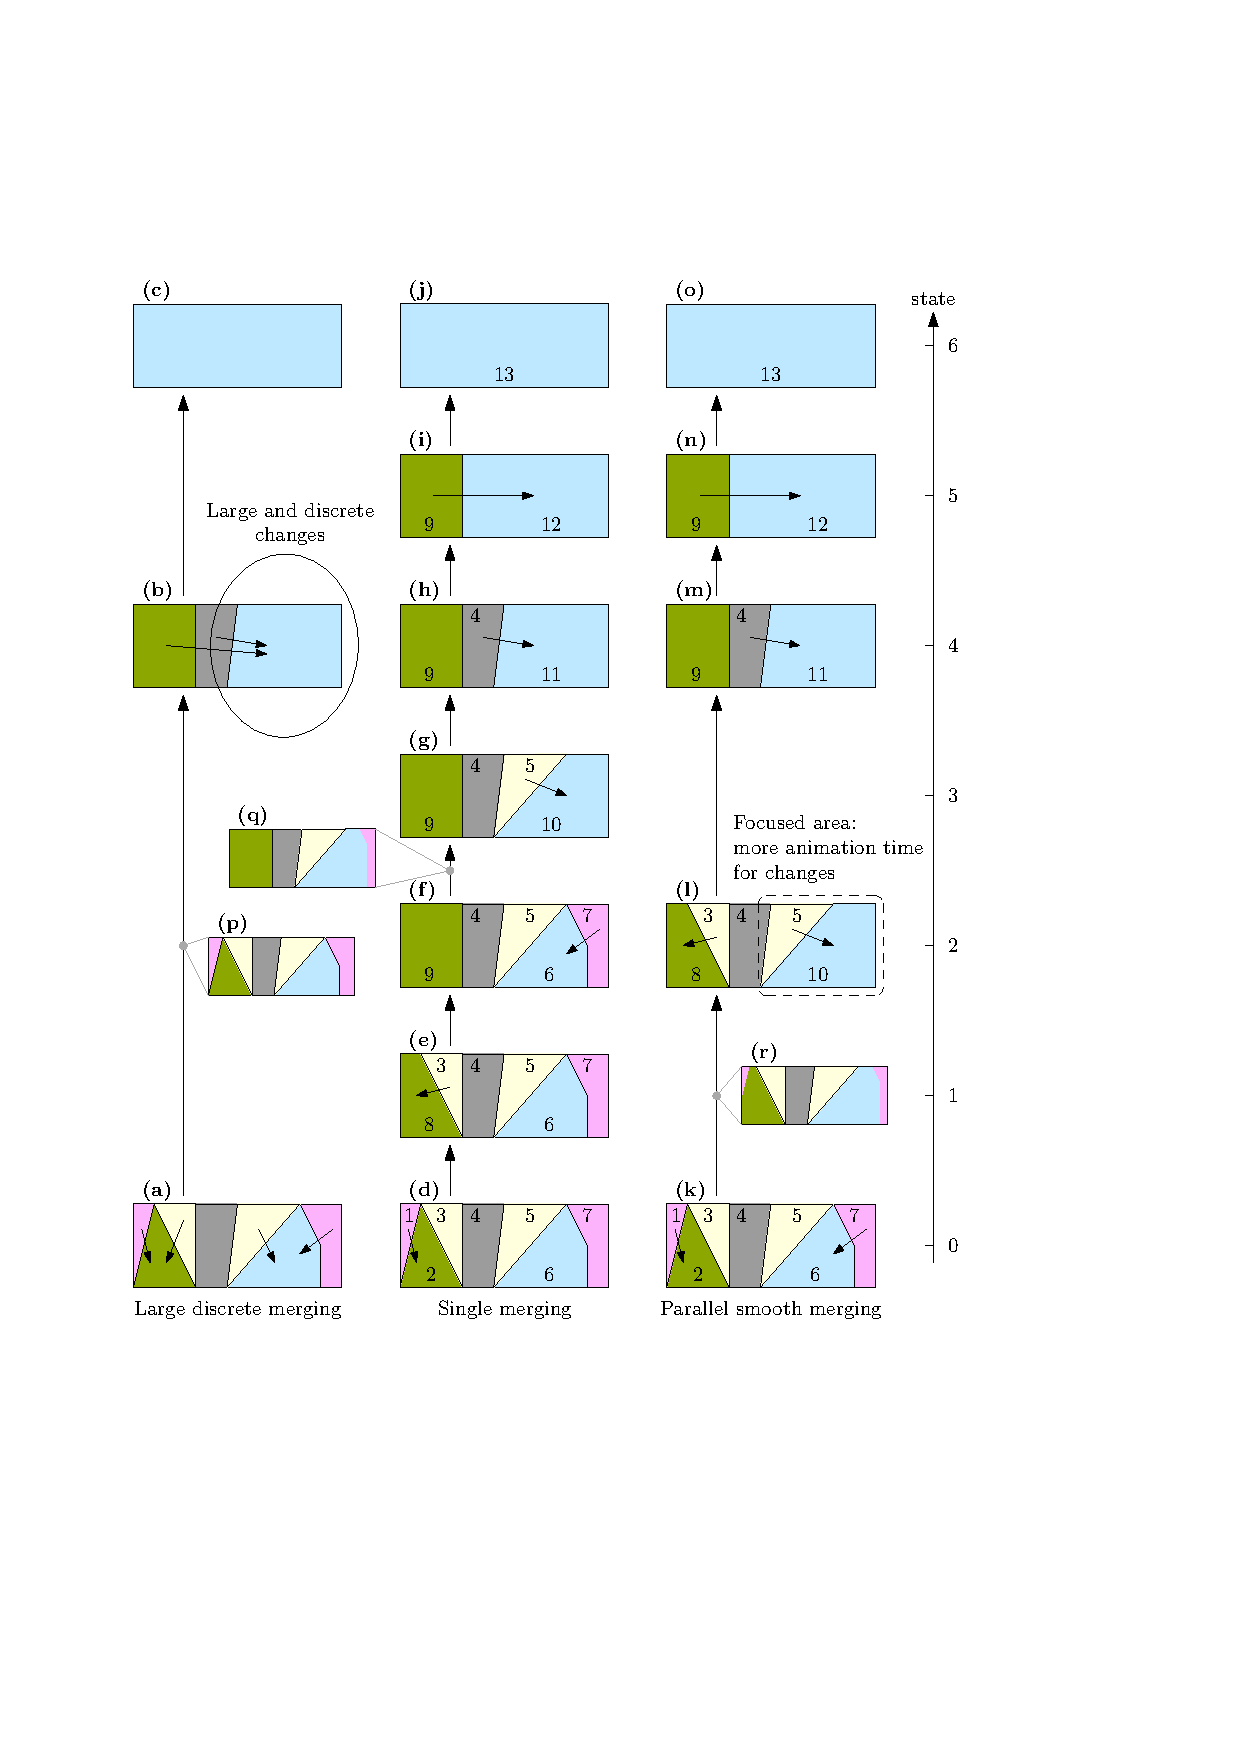
\includegraphics[page=1,scale=0.99]{introduction}
\caption{A comparison of different scale-transition strategies for zooming out.
Each arrow inside the subfigures indicates that 
an area will be merged into another one.
The arrow in the right-hand side indicates the states of zooming out,
which is related to the transition duration.
%
(a--c): All changes are processed in one go.
(d--j): All changes are sequenced one by one rapidly.
(k--o): Changes are grouped, resulting in more animation duration for every change.
%where smooth and parallel changes going on can be found in figure~(r);
%digital map with smooth and parallel generalization operations.
%
The ellipse shows an example place where large and discrete change happens.
The dashed polygon shows the place where a user focuses;
the user has about twice of the duration 
to perceive the merging of the pink area, \ie~figures (k--l),
comparing to figures (f--g).
The numbers are ids of the faces.
}
\label{fig:intro}
\end{figure}



\begin{figure}
\centering
\begin{subfigure}[t]{0.48\textwidth}
\centering
\includegraphics[page=4,width=0.95\linewidth]{methodology}
\caption{The SSC of the single merging shown in \figs\ref{fig:intro}d--j.
    If slicing the SSC with a horizontal plane at $z$-coordinates~$0$, 
    $100$, $200$, $300$, $400$, $500$, and~$600$,
    then we get \figs\ref{fig:intro}d--j.
    If slicing it at $z$-coordinate~$250$,
    then we get \fig\ref{fig:intro}q.}
\end{subfigure}
\hfill
\begin{subfigure}[t]{0.48\textwidth}
\centering
\includegraphics[page=5,width=0.95\linewidth]{methodology}
\caption{The SSC of the parallel merging shown in \figs\ref{fig:intro}k--o.    
    If slicing the SSC with a horizontal plane at $z$-coordinates~$0$, 
    $200$,  $400$, $500$, and~$600$,
    then we get \figs\ref{fig:intro}k--o.
    If slicing it at $z$-coordinate~$100$,
    then we get \fig\ref{fig:intro}r.}
\end{subfigure}
\caption{
The content of each of the SSCs is stored in an OBJ file,
and each of the figures is generated by displaying the OBJ file
in software ParaView.
The $z$-coordinates are $100$ times of the state values in \fig\ref{fig:intro}.
We did this multiplication so that the contents can be better observed;
otherwise, the two SSCs will be very short when displayed in ParaView.
The faces are displayed with opacity~$0.8$ so that we can see some faces behind.
Smooth animations of zooming out are obtained by
slicing the SSCs from bottom to top.
Note that both SSCs have exactly same bottom and top content 
(also with same $z$-coordinates). 
In the left SSC, only one merging event is happening 
at a specific state ($z$-dimension), 
while in the right SSC multiple merging events may happen at the same state.
}
\label{fig:ssc}
\end{figure}


%
%\begin{figure}
%\centering
%\begin{subfigure}[t]{0.48\textwidth}
%\centering
%\includegraphics[page=4,width=0.95\linewidth]{methodology}
%\caption{}
%\end{subfigure}
%\hfill
%\begin{subfigure}[t]{0.48\textwidth}
%\centering
%\includegraphics[page=5,width=0.95\linewidth]{methodology}
%\caption{}
%\end{subfigure}
%\caption{
%
%}
%\label{fig:ssc}
%\end{figure}

%\begin{figure}
%\centering
%%
%\subfigure[The SSC of the single merging shown in \figs\ref{fig:intro}d--j.
%    If slicing the SSC with a horizontal plane at $z$-coordinates~$0$, 
%    $100$, $200$, $300$, $400$, $500$, and~$600$,
%    then we respectively get \figs\ref{fig:intro}d--j.
%    If slicing it at $z$-coordinate~$250$,
%    then we get \fig\ref{fig:intro}q.]{
%\resizebox*{0.48\textwidth}{!}{\includegraphics[page=4,width=0.95\linewidth]{methodology}}}\hfill
%%
%\subfigure[The SSC of the parallel merging shown in \figs\ref{fig:intro}k--o.    
%    If slicing the SSC with a horizontal plane at $z$-coordinates~$0$, 
%    $200$,  $400$, $500$, and~$600$,
%    then we respectively get \figs\ref{fig:intro}k--o.
%    If slicing it at $z$-coordinate~$100$,
%    then we get \fig\ref{fig:intro}r.]{
%\resizebox*{0.48\textwidth}{!}{\includegraphics[page=5,width=0.95\linewidth]{methodology}}}
%%
%\caption{The content of each of the SSCs is stored in an OBJ file,
%and each of the figures is generated by displaying the OBJ file
%in ParaView~5.8.0.
%The $z$-coordinates are $100$ times of the state values in \fig\ref{fig:intro}.
%We did this multiplication so that the contents can be better observed;
%otherwise, the two SSCs will be very short when displayed in ParaView.
%The faces are displayed with opacity~$0.8$.
%Smooth animations of zooming out are obtained by
%slicing the SSCs from bottom to top.} 
%\label{fig:ssc}
%\end{figure}


When users zoom on maps, 
they do not want to wait for too long to see the map at the desired scale.
On a real map, however, 
many changes must be processed to arrive at the desired scale.
If the changes are processed one by one 
(\eg~\figs\ref{fig:intro}d--j),
then the animation duration for each change has to be very short.
Users may still lose their context because of the fast changes.
For example, a user may get the impression of
a shock change from \fig\ref{fig:intro}f to \fig\ref{fig:intro}h
(without the intermediate state of \fig\ref{fig:intro}g)
even when the three areas on the right-hand side of \fig\ref{fig:intro}f
are merged smoothly.
To provide users with more gradual impression, 
we parallel the generalization operations.
For example, we should split or merge the relatively unimportant areas,
and we should simplify the boundaries of the areas.
If we select some of the generalization operations
and process them in parallel,
then each operation has more time to take place 
than the operations are processed one after another.
Moreover, if the selected operations are
fairly evenly distributed on the whole map, 
then there may be only a limited number of operations 
happening in users' focused region.
We assume that it is easier for users to keep track of their interested areas
when fewer operations take place longer on the focused region.
As for the operations happening outside the focused region,
they can be ignored because 
they are not interesting to map users at the moment.
In this paper, we focus on paralleling merging operations.\footnote{%
See the map at
\url{https://congengis.github.io/webmaps/2020/05/merge/example-parallel-merging/}.}
For example, in the focused area, there is only one merging operation 
from \fig\ref{fig:intro}l to \fig\ref{fig:intro}m,
whereas there are two merging operations  
from \fig\ref{fig:intro}f to \fig\ref{fig:intro}h;
a user will have about twice of the duration to perceive the changes of the former
(see duration assignment in \sect\ref{sec:zooming_duration}).\footnote{%
A comparison of the single merging (left) 
and the parallel merging (right) is at
\url{https://congengis.github.io/webmaps/2020/05/merge/example-parallel-merging/comparer.html}, 
where the slider at the left-hand side can be 
moved to adjust the canvases of the two maps.}


This paper is organized as follows.
\sect\ref{sec:realted_work} reviews some related work.
Our methodology is presented in \sect\ref{sec:methodology}.
We show a case study in \sect\ref{sec:case_study}.
Finally, \sect\ref{sec:concluding_remarks} draws the conclusion
and present our future work.


\section{Related work}
\label{sec:realted_work}


\citet[\chap2]{Peng2019Thesis} tried to 
find an optimal sequence to merge area objects 
based on the \Astar algorithm or an integer linear program.
A comparison to a greedy algorithm showed that 
the \Astar algorithm improves the quality of the merging sequences
in the sense of the class changes and the area compactnesses.
\Citet{vanOosterom2014Support} pointed out that 
sequentially processing generalization operations 
may result in no change at some locations in a zooming duration, 
which seems unnatural.
Therefore, they suggested paralleling the generalization operations,
but no implementation, testing, or assessment of the idea was provided.
%Then, one question is how many operations 
%should be paralleled for a given scale.
\citet{Thiemann2018LandCover} proposed a chain of operators 
to generalize a land-cover map.
In the chain of processing area objects, 
they integrated cleaning, dissolving, splitting, 
aggregating, reclassifying, and simplifying. 

\Citet{vanOosterom2014Support} 
explained the concept of the space-scale cube (SSC).
At the bottom of the SSC is a detailed topographic map,
and all the area objects extrude along the $z$-axis.
In the SSC, an area on the map becomes a polyhedron, and
the common boundary of two areas is a vertical wall.
Whenever a generalization operation happens, 
the extrusions of the involved areas stop;
then, the newly generated areas take the place and start to extrude.
On this basis, the map at any scale can be generated by slicing the SSC 
with a horizontal plane at a corresponding $z$-coordinate.
That is to say, the scale becomes the third dimension of the map in the SSC
(\eg~\fig\ref{fig:ssc}).
Furthermore, they represented the smooth tGAP in the SSC.
A typical example of the smooth generalization operation is that 
an area merges with another one by gradually expanding over it.
In the SSC of the smooth tGAP, 
the wall starts to tilt when the expansion begins.
Based on the SSC, \citet{Meijers2020Web} explained the principles of 
implementing a web map of area objects.
They showed how to request only a part of a large dataset of a vario-scale map.
They made chunks of the SSC data
so that they were able to send only the chunks relevant 
to users' interested place.
They showed how to efficiently slice the SSC 
to output a web map at a given scale 
using the GPU at the client side using WebGL in the browser.
In addition to slicing the SSC with a horizontal plane,
they could also slice the SSC with a curly surface 
to have a locally more detailed map
or with a tilted surface to have a perspective view.
To build an SSC, \citet{Suba2014Merge} proposed three methods 
to merge a pair of areas in a gradual manner, 
which are the \emph{Single flat plane}, 
the \emph{Zipper}, and the \emph{Eater}.
Basically, the \emph{winner} area gradually expands over the \emph{loser} area.
We will use the \emph{Eater} because it works for all kinds of polygons,
while the other two methods have limitations for some special cases.
For example, the two other methods do not work for some concave polygons.
\citet{Huang2016Webmap} pointed out that
the effort of implementing online maps 
had been spent mainly on preparing data on the server side.
They studied the communication of map data 
between the server side and the client side.
They proposed different strategies of assigning 
the work of processing map data
according to the machine abilities of the clients.

\citet{Suba2016Road} continuously generalized a planar map of road network.
In each step, they process the least important face.
Taking into account the local condition of the face
(\eg~no compatible neighbor at the same side of the road),
they may take different decisions for the face: 
put it back with a higher importance, collapse it, 
or merge it into an adjacent face.
In addition to the map generalization, 
they also made statistics of the number of faces,
the area of faces, the number of road faces, the number of road edges,
and the number of operations (merge and split) 
when the map scale is decreasing.
These statistics can be good indications 
for (continuous) map generalization.
\citet{Huang2017Matrix} utilized a matrix to guide 
both pruning rivers and removing vertices for a river network, 
where the rows and the columns respectively represent
the rivers and the vertices.
According to the matrix, 
they were able to decide which rivers and vertices 
should remain for a given scale.
To that purpose, they proposed a method 
to compute how many rivers and vertices 
should be kept according to that given scale.





%\citet{Dumont2020MultiScale}
%\citet{Meijers2015Parallel}

%


\section{Methodology}
\label{sec:methodology}


In order to provide smooth merging
so that map users can easily keep track of their interested areas,
we merge by gradually expanding an area over another area
(see \fig\ref{fig:intro}r).
This expansion can be realized 
by slicing the space-scale cube (SSC) shown in
\fig\ref{fig:ssc}b.
%For example, \figs\ref{fig:smooth_merging}a,
%\ref{fig:smooth_merging}b, and \ref{fig:smooth_merging}c
%are respectively obtained from slicing the cube 
%at the bottom, the middle, and the top.
The details of slicing an SSC are illustrated in \citet{Meijers2020Web}.
The SSCs of \fig\ref{fig:ssc} was built 
based on the \emph{Eater} of \citet{Suba2014Merge}.
\fig\ref{fig:intro}r shows our solution of
gradually expanding an area over the other area.
Our strategy of presenting the static boundary (\ie~the exterior one) 
is that we store the polylines and 
draw them with width, 
where the width is computed according to the map scale on the fly.
We do not draw the common boundary of 
a pair of areas that are being merged
so that it is easy for map users 
to identify the pairs of areas in transition. 



We define an \emph{event} as a single generalization operation, 
such as merging an area into a neighbor.
For example, \fig\ref{fig:intro}e is obtained from 
\fig\ref{fig:intro}d by processing one merging event.
Similarly, \fig\ref{fig:intro}l is obtained from 
\fig\ref{fig:intro}k by processing two merging events.
We define a \emph{step} as 
a set of events happening at the same animation duration.
For example, 
\fig\ref{fig:intro}e is obtained from 
\fig\ref{fig:intro}d by processing a step with one merging event.
\fig\ref{fig:intro}l is obtained from 
\fig\ref{fig:intro}k by processing a step with two merging events.
In our method, a step is completely processed 
before the next step takes place (all sequential).
We define a \emph{state} as the point when a step starts or finishes.
For example, there are seven states 
in the merging sequence of \figs\ref{fig:intro}d--j
(\ie~states 0, 1, 2, 3, 4, 5, and 6, from bottom to top)
and five states in the merging sequence of \figs\ref{fig:intro}k--o 
(\ie~states 0, 2, 4, 5, and 6).
The value of a state is also the total number of events processed so far.


We require that 
the area objects involved in different merging events of the same step 
must not be neighbors, 
which makes the merging events independent from each other.
There are two benefits of this independency.
First, it is easy to maintain the topology of the map.
When a pair of areas have been merged, 
we must update the common boundaries with the surrounding adjacent areas.
If an adjacent area is involved in another merging event,
then it is complicated to update the adjacent area's boundaries
for the two merging events.
Second, users can keep track of their interested areas more easily
than merging several areas into a single one.
In order to realize the requirement,
we block the neighbors of the areas once we have found an event.
We show a greedy algorithm to find the parallel merging events for each step
in \sect\ref{sec:greedy_algo}.
Then, we integrate the events into the tGAP databse tables
(\sect\ref{sec:integrate_tgap}),
followed by integrating the events into the SSC 
(\sect\ref{sec:integrate_ssc}).
In \sect\ref{sec:snap}, we show how to snap the zooming to valid states
to avoid half-way merging animation 
as stopping halfway will result in showing slivers in a static state.
In \sect\ref{sec:zooming_duration}, we define 
the animation duration of zooming from one state to another state.



\subsection{A greedy algorithm}
\label{sec:greedy_algo}

In the greedy algorithm, 
we need to obtain the most compatible neighbor for a given area.
There are many ways of defining the most compatible neighbor.
For example, \citet{Cheng2006} proposed three choices, i.e.,
the neighbor has the largest size, 
shares the longest boundary with the least important area,
or has the closest class to the least important area. 
\citet{Peng2017AStar} proposed that 
the most compatible neighbor should have a close class
to the least important area
and the combination of the two areas should be compact;
they defined the class distance based on a binary tree
according to the codes of the classes.
We define the importance and the compatibility as
the same as \citet{vanOosterom2005,vanPutten1998NewGAP}.
That is, the importance of an area is the multiplication 
of its size and its class weight.
The compatibility value between a pair of areas is 
the multiplication of the common boundary's length and 
the class similarity of the two areas.
\appx\ref{appx:create_tables} shows our implementation of
computing the weight values and the class similarities.



\fig\ref{fig:greedy_framework} shows the flowchart of our greedy algorithm.
The process starts with state~$s=0$ and a detailed map of area objects, $|M_0|$.
Parallel parameter~$r_\mathrm{parallel}$ specifies 
the proportion (\ie~percentage, when multiplied by~$100$) of area objects that
we expect to merge parallelly.
As a value of percentage, 
$r_\mathrm{parallel}$ is in the range from~$0\%$ to~$100\%$,
which means~$r_\mathrm{parallel} \in [0,1]$.
Expression~$|M_s|$ denotes the number of area objects of the map at state~$s$.
If there is more than one area ($|M_s|>1$),
then we start finding merging events.
We first compute the number of areas that we expect to merge by
\begin{equation}
\label{eq:n_target}
n_\mathrm{target} =
\lceil r_\mathrm{parallel} \cdot |M_s| \rceil,
\end{equation}
where the ceiling function guarantees~$n_\mathrm{target}\ge 1$.
That is to say, we find at least one event for each step.
When~$n_\mathrm{target} > 1$, however,
we cannot always find~$n_\mathrm{target}$ events
because some areas may be blocked as explained before
(also see \fig\ref{fig:blocked_polygons}).
Therefore, we use variable~$n_\mathrm{event}$
to represent the number of events that actually happened within the step. 


\begin{figure}[tb]
\centering
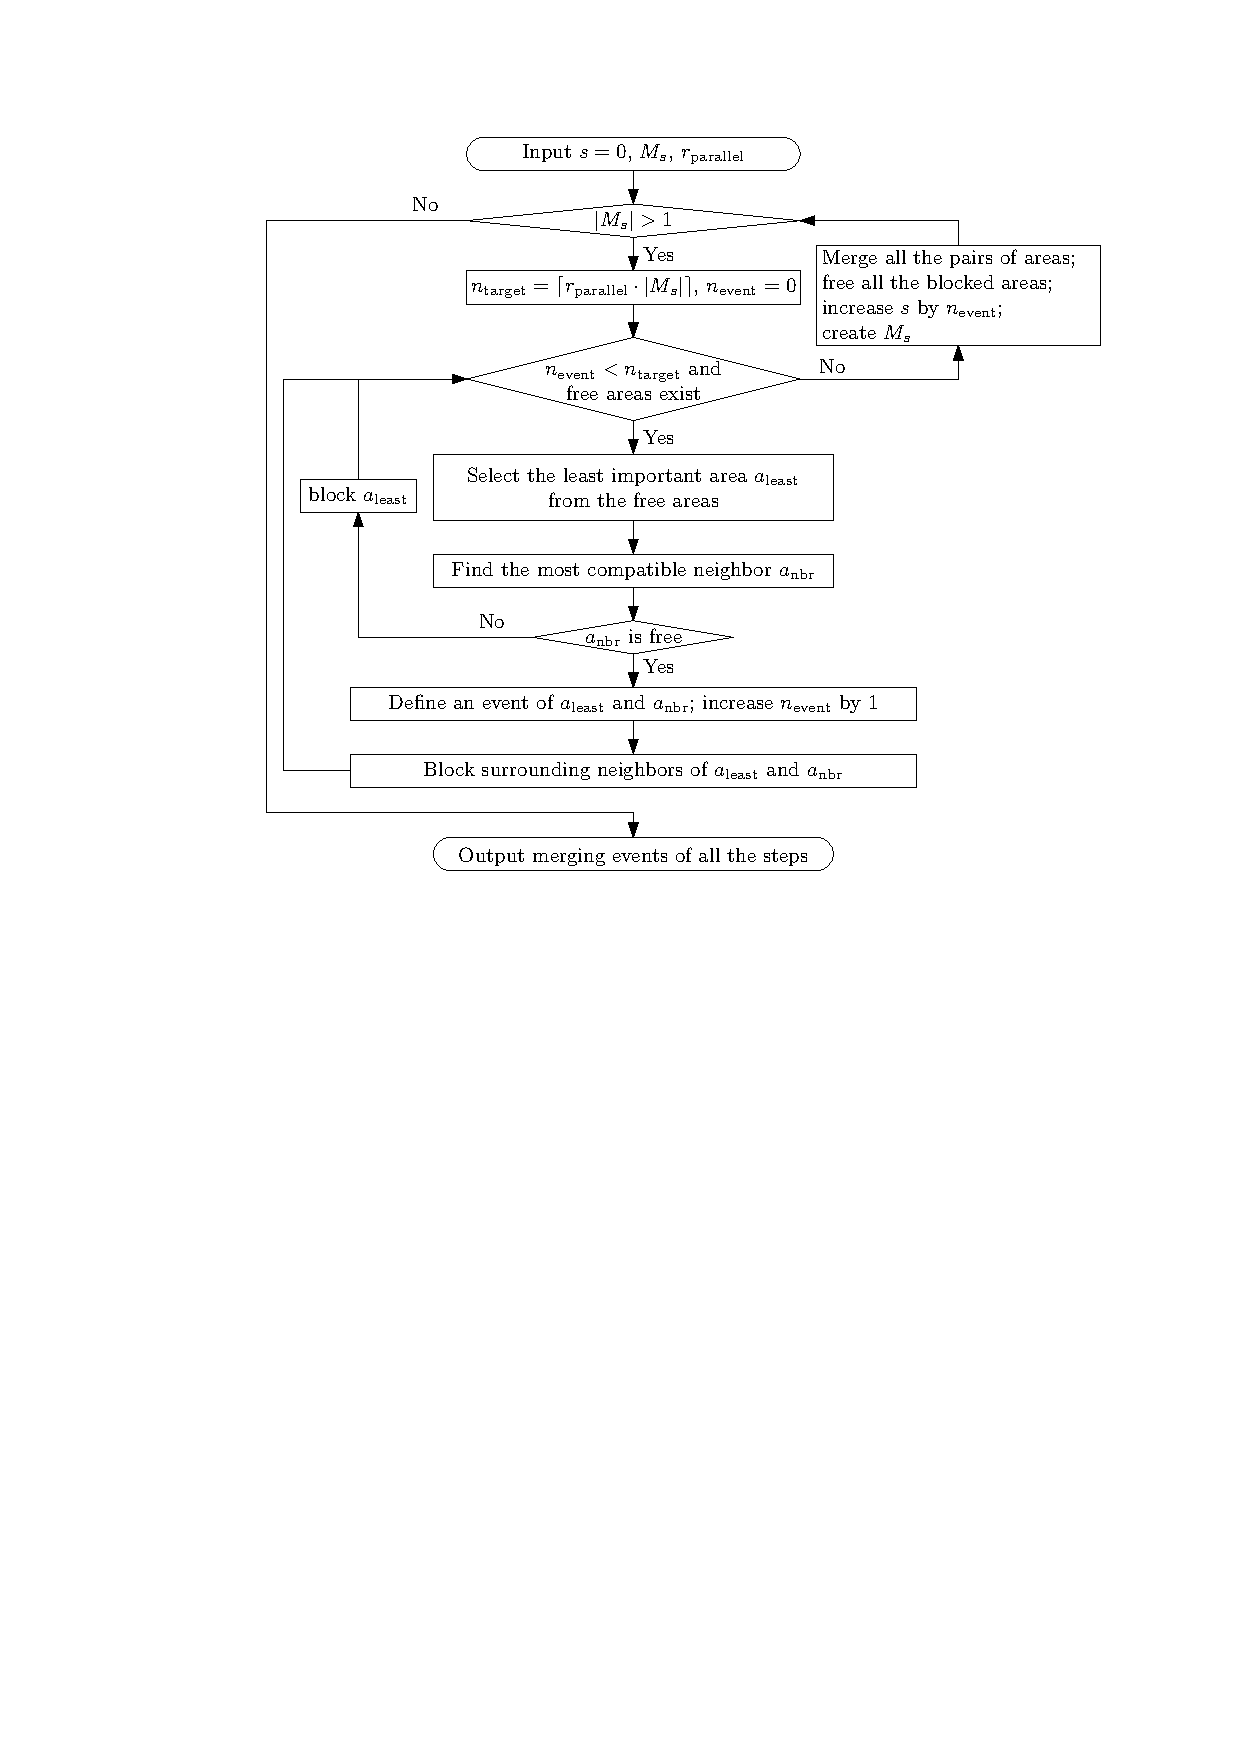
\includegraphics[page=1]{methodology}
\caption{The flowchart of our greedy algorithm.
}
\label{fig:greedy_framework}
\end{figure}


\begin{figure}[tb]
\centering
\includegraphics[page=2]{methodology}
\caption{The process of finding parallel merging events for a step.
    (a) From all the free areas,
	the least important one is selected to merge into
	its most compatible neighbor.
    The arrow indicates the merging.
	Then the surrounding areas are blocked (marked by the crosses).
    Note that the area shares only a vertex with the least important area 
    is not blocked.
	(b) Next, the least important area from the remaining free areas
	is selected to merge with the most compatible neighbor,
	and the surrounding areas are also blocked.
}
\label{fig:blocked_polygons}
\end{figure}

If we have not found $n_\mathrm{target}$ events 
($n_\mathrm{event} < n_\mathrm{target}$)
and there are still free areas,
then we go on looking for merging events.
We select the least important area~$a_\mathrm{least}$
from the free areas.
An area is \emph{free} if 
it is not involved in an event and is not blocked.
We also find~$a_\mathrm{least}$'s 
most compatible neighbor~$a_\mathrm{nbr}$.
If area~$a_\mathrm{nbr}$ is also free, 
we define an event of areas~$a_\mathrm{least}$ and~$a_\mathrm{nbr}$.
Then, we increase the number of events, $n_\mathrm{event}$, by 1.
We block the surrounding neighbors of~$a_\mathrm{least}$ and~$a_\mathrm{nbr}$
(see \fig\ref{fig:blocked_polygons}a).
If area~$a_\mathrm{nbr}$ is not free,
then it must be blocked because of the previously found events.
In this case, we block $a_\mathrm{least}$ for now
so that areas~$a_\mathrm{least}$ and~$a_\mathrm{nbr}$ 
may merge in the next step.
Then, we continue to find more merging events and to block more areas
(see \fig\ref{fig:blocked_polygons}b).

If we have found~$n_\mathrm{target}$ events 
or there is no free area anymore,
then finding merging events of the step finishes.
We parallelly merge all the pairs of areas of the found events
to generate new areas,
free all the blocked areas,
increase state~$s$ by value~$n_\mathrm{event}$,
and create map~$M_s$ based on the new areas and the freed areas.
Then, finding merging events for the next step starts.
This iteration of finding completes 
until there is only one area left on the map ($|M_s|=1$).
The merging events will be stored as records in tGAP database tables
(see \fig\ref{fig:uml_tgap}).
\figs\ref{fig:intro}k--o show a sequence of four merging steps
obtained by our greedy algorithm,
where parallel parameter~$r_\mathrm{parallel}$ is set to~$0.3$
(Note that this is an extremely high value, 
just used to explain the principle in an artificial simple example).



\begin{figure}[tb]
\centering
\includegraphics[page=3]{methodology}
\caption{The UML diagram of the classes stored in tGAP databse tables.
This diagram is a slightly improved version of \citet[\p159]{Meijers2011Thesis}.
In the face table, property \emph{pip\_geometry} 
stores a point (usually the center) in the face (polygon).
The geometry of a face can be obtained by calling function \emph{getGeometry()}.
We do not store the face geometry because we want to avoid redundancy,
as the edges already stores the sequences of points.
}
\label{fig:uml_tgap}
\end{figure}


\subsection{Integrating the parallel events into the tGAP databse tables}
\label{sec:integrate_tgap}

\citet[\p159]{Meijers2011Thesis} designed three tables 
to record the information of
faces, edges, and face hierarchies, 
which together form a tGAP.
For example, the face table contains columns \emph{face\_id}, 
\emph{imp\_low}, \emph{imp\_high}, \emph{imp\_own},
\emph{feature\_class}, \emph{area}, and \emph{mbr\_geometry}.
We add columns \emph{state\_low} ($s_\mathrm{low}$) 
and \emph{state\_high} ($s_\mathrm{high}$) into the table 
so that it is easy to see when a face should appear or disappear 
(see \tabls\ref{tbl:face_tgap}a and~\ref{tbl:face_tgap}b,
where all other columns, except face\_id, are hidden).
For zooming out, a face should appear, 
from the merging of two faces,
when the slicing arrives at the low state.
When the slicing arrives at the high state,
the face should have been merged with another area.
Comparing between the tables of single merging 
(\figs\ref{fig:intro}d--j)
and parallel merging (\figs\ref{fig:intro}k--o),
we observed some differences of the values.
For example, the $s_\mathrm{high}$ values of faces~1 and~2 are changed from~1 to~2
(see \tabl\ref{tbl:face_tgap}).
Also, the $s_\mathrm{low}$ value of face~8 is changed from~1 to~2
(see \tabl\ref{tbl:face_tgap}).
Similarly to the face tables, 
the columns and records of both the edge table and the face-hierarchy table 
will be changed accordingly.


\begin{table}[tb]
\caption{Some columns of the face tables. 
    Columns~$s_\mathrm{low}$, $s_\mathrm{merge}$, 
    and~$s_\mathrm{high}$ show the states 
    when the faces appear, when the faces start to disappear, and
    when the faces completely disappear.    
    In table~(b), the different values from table~(a) are underlined.
    Column~$s_\mathrm{merge}$ is not really stored in the database.
    We show the column so that it is easy to see the differences 
    between the $s_\mathrm{low}$ values and the $s_\mathrm{merge}$ values.
    }
\label{tbl:face_tgap}
\begin{subtable}{0.48\textwidth}
\caption{The face table of the single merging 
    shown in \figs\ref{fig:intro}d--j.}
\centering
\begin{tabular}{cccc}
\toprule
$f_\mathrm{id}$& $s_\mathrm{low}$    & $s_\mathrm{merge}$ & $s_\mathrm{high}$ \\ \midrule
1       &     0         &     0         &     1       \\
2       &     0         &     0         &     1       \\
3       &     0         &     1         &     2       \\ 
4       &     0         &     4         &     5       \\
5       &     0         &     3         &     4       \\
6       &     0         &     2         &     3       \\         
7       &     0         &     2         &     3       \\
8       &     1         &     1         &     2       \\
9       &     2         &     5         &     6       \\         
10      &     3         &     3         &     4       \\
11      &     4         &     4         &     5       \\ 
12      &     5         &     5         &     6       \\ 
13      &     6         &    ---        &    ---      \\
\bottomrule
\end{tabular}
\end{subtable}
%
\hfill
%
\begin{subtable}{0.48\textwidth}
\caption{The face table of the parallel merging 
    shown in \figs\ref{fig:intro}k--o.}
\centering
\begin{tabular}{cccc} %\underbar{2}
\toprule
$f_\mathrm{id}$ & $s_\mathrm{low}$   & $s_\mathrm{merge}$ & $s_\mathrm{high}$ \\ \midrule
1       &     0         &     0         &\underbar{2} \\
2       &     0         &     0         &\underbar{2} \\
3       &     0         & \underbar{2}  &\underbar{4} \\ 
4       &     0         &     4         &     5       \\
5       &     0         & \underbar{2}  &     4       \\
6       &     0         & \underbar{0}  &\underbar{2} \\         
7       &     0         & \underbar{0}  &\underbar{2} \\
8       & \underbar{2}  & \underbar{2}  &\underbar{4} \\
9       &     2         &     5         &\underbar{6} \\         
10      & \underbar{4}  & \underbar{2}  &\underbar{4} \\
11      &     4         &     4         &     5       \\ 
12      &     5         &     5         &     6       \\ 
13      &     6         &    ---        &    ---      \\
\bottomrule
\end{tabular}
\end{subtable}
\end{table}


\subsection{Integrating the parallel events into the SSC}
\label{sec:integrate_ssc}

Recall that we merge a pair of areas by expanding over 
the less important area from the neighbor.
The Eater of \citet{Suba2014Merge} is used to 
triangulate the less important area and to tilt the triangles.
Then the tilted triangles are integrated into the SSC
(see \fig\ref{fig:ssc})
so that we can slice the SSC to achieve smooth merging.
For the case of single merging,
if a pair of areas have state-high value~$s_\mathrm{high}$,
then the merging animation 
always starts at state~$s_\mathrm{merge}=s_\mathrm{high}-1$
(see \tabl\ref{tbl:face_tgap}a).
The less important area completely disappears
at state~$s_\mathrm{high}$.
In the face table, a row will be added to record the new area, 
and its $s_\mathrm{low}$ value will be the previous~$s_\mathrm{high}$ value.
The new area takes the combined place of the pair of areas.
Take \ref{fig:intro} as an example, 
area~1 is merged into area~2 (\figs\ref{fig:intro}d), 
and area~8 is generated to take the combined place (\figs\ref{fig:intro}e).
The tilted triangle is the one spans 
from~$z= 0$ to~$z=100$ (\ie~from state~0 to state~1)
in \fig\ref{fig:ssc}a.
In \tabl\ref{tbl:face_tgap}a, 
the~$s_\mathrm{low}$ value of area~8 is 1,
which is the~$s_\mathrm{high}$ values of areas~1 and~2.
%Note that the state\_low values of the two areas do not matter 
%because those values respectively indicate the states that
%the two areas appear;
%those values can be much smaller 
%than value~$s_\mathrm{high}-1$.

For the case of parallel merging,
if a step consists of~$n_\mathrm{event}$ events and 
the step finishes at state~$s_\mathrm{high}$, then the step starts 
at state~$s_\mathrm{merge}=s_\mathrm{high} - n_\mathrm{event}$.
The reason is that if the~$n_\mathrm{event}$ events 
would happen sequentially (\ie~single merging),
then they would take place 
from state~$s_\mathrm{high} - n_\mathrm{event}$ to state~$s_\mathrm{high}$.
When all the events take place parallelly in the same step, 
each of the events can share its merging duration.
%there is a less important area in each of the parallel events of a merging step.
%If the number of parallel events is~$n_\mathrm{event}$,
%then there are~$2n_\mathrm{event}$ areas 
%with the same state\_high value, say,~$s_\mathrm{high}$
%because each merging event involves two areas.
%The merging animations of all the parallel events
%start at state~$s_\mathrm{merge}=s_\mathrm{high} - n_\mathrm{event}$
%and finishes at state~$s_\mathrm{high}$.
%By definition, the parallel events of a merging step 
%happen during the same animation time.
%In other words, the areas involved in those parallel events have 
%the same state\_merge value ($s_\mathrm{merge}$) and 
%the same state\_high value ($s_\mathrm{high}$).
%The reverse is also true.
%If some areas have the same state\_high value,
%then those areas happen during the same animation time 
%(involved in the parallel events of the same step).
%The reason is that, according to our requirement,
%a step can start only when the previous step stops.
%Thus, the merging events finishing at the same state cannot from different steps.
%of these areas 
%will finish at state~$s_\mathrm{high}$,
%and no merging event will start earlier or later than state~$s_\mathrm{merge}$
%because we required that the next step starts only when a step stops.
%Given the fact that the merging duration for zooming 
%between states~$s_\mathrm{merge}$ and~$s_\mathrm{high}$ is fixed,
As a result,
each of the parallel events has more time to take place
than the events would happen sequentially.
In other words, for a merging step,
each of the events has more time to take place 
if there are more parallel events.

In order to build the SSC for parallel merging,
we need the~$s_\mathrm{merge}$ value for each of the merging steps
so that we know from which state 
the triangles of the less important areas should be tilted.
A simple way is to add a column, say, $s_\mathrm{merge}$
into the face table during generating the tGAP, 
as done in \tabl\ref{tbl:face_tgap}.
Then, the states of starting merging can be recorded into the column.
However, we would like to avoid unnecessary columns to save storage.
Therefore, we compute~$s_\mathrm{merge}$ values 
based on the~$s_\mathrm{high}$ values
on the fly when building the SSC.
As an event involves two areas,
the number of events finishing at state~$s_\mathrm{high}$ can be calculated by
\begin{equation*}
\label{eq:n_event_state}
n_\mathrm{event} (s_\mathrm{high}) = 
\frac{\sum\limits_{s \in S_\mathrm{high}} [s=s_\mathrm{high}]}{2},
\end{equation*}
where notation~$S_\mathrm{high}$ denotes the set of values
recorded in column~$s_\mathrm{high}$ of the face table
(\eg~\tabl\ref{tbl:face_tgap}b).
Expression~$[s=s_\mathrm{high}]$ returns~$1$ if the two values are equal 
and returns~$0$ otherwise.
As illustrated before, the state at which the parallel merging starts 
can be computed by
\begin{equation*}
\label{eq:s_merge_state}
s_\mathrm{merge} (s_\mathrm{high}) = s_\mathrm{high} - n_\mathrm{event} (s_\mathrm{high}).
\end{equation*}



Take the case of \tabl\ref{tbl:face_tgap}b for example,
we have~$S_\mathrm{high} = \{2, 2, 4, 5, 4, 2, 2, 4, 6, 4, 5, 6\}$, 
$n_\mathrm{event} (4) = 2$, and~$s_\mathrm{merge} (4) = 2$.
Therefore, there are two merging events finishing at state~$4$,
\ie~event of merging area 3 into area~8 and 
event of merging area~5 into area~10 
(also see \figs\ref{fig:intro}l and~\ref{fig:intro}m).
The merging animation takes place from state~$2$ to state~$4$.
This merging can be also observed from 
the two tilted triangles spanning from~$z = 200$ to~$z = 400$ 
in \fig\ref{fig:ssc}b.
In merging sequence of \figs\ref{fig:intro}d--j, 
the animation of merging area~3 into area~8 
takes place from state~$1$ to state~$2$
(also see the tilted triangle spanning from~$z = 100$ to~$z = 200$ 
in \fig\ref{fig:ssc}a), and 
the animation of merging area~5 into area~10
takes place from state~$3$ to state~$4$
(also see the tilted triangle spanning from~$z = 300$ to~$z = 400$ 
in \fig\ref{fig:ssc}a).
As a result, the animation duration of merging area~3 into area~8 of 
sequence \figs\ref{fig:intro}k--o
is almost twice as that of sequence \figs\ref{fig:intro}d--j.
We say \emph{almost} because the animation duration is also dependent on 
the current state of the map
(see \sect\ref{sec:zooming_duration}).


\subsection{Snapping to a valid state}
\label{sec:snap}

For a zooming action based on the SSC, 
we always snap the map to a valid state.
In this way, users will not see a merging operation stops half-way
and will not see transition artifact (such as slivers).
Take the sequence of \fig\ref{fig:intro}k--o for example, 
the merging animation should stop at 
either \ref{fig:intro}k or \ref{fig:intro}l,
but not at \ref{fig:intro}r.
Note that some states are not valid because of the parallel events.
For example, state~$1$ is not valid 
for the sequence of \fig\ref{fig:intro}k--o.
In that example, the list of valid states 
is~$S_\mathrm{valid} = [0, 2, 4, 5, 6]$.
In order to snap to one of the valid states after a zooming operation,
we have to communicate them to the client side. 
There are multiple options. 
The most simple one assumes that, 
during the creation of the parallel SSC, 
we can always perform the~$n_\mathrm{target}$ number of events in all steps. 
In that case, we just have to communicate 
the number of areas and the ratio~$r_\mathrm{parallel}$. 
In case of high value ratios (\eg~$r_\mathrm{parallel} > 0.01$), 
this assumption may be incorrect. 
We then have to communicate the valid states by sending them explicitly. 
Because this list may get rather large,
we only send exceptions.
\appx\ref{appx:communicate_valid_states} shows the details of the technique.
As a result, the list of valid states~$S_\mathrm{valid}$ is sent to the client side.


According to how much a user has zoomed,
the target scale, say, $1:S_\mathrm{t}$ can be computed.
%According to \citet{Huang2016Webmap},
%the number of merging events that should be processed can be computed by
\citet{Huang2016Webmap} suggested that 
the average density of the original map should be preserved 
for a smaller-scale map.
Their suggestion is based on the assumption that 
the area density of the base map is well designed, which is reasonable.
We use variable~$A_\mathrm{real}$ to denote the total areal size of 
all the area objects in reality.
Then, the size on screen at scale~$1:S_\mathrm{t}$ 
is~$A_\mathrm{real} \big/ S^2_\mathrm{t}$.
In order to keep the density, we require
\begin{equation}
\label{eq:equal_density}
\frac{N_\mathrm{b}}{A_\mathrm{real} \big/ S^2_\mathrm{b}} =
\frac{N_\mathrm{b}-E_\mathrm{t}}{A_\mathrm{real} \big/ S^2_\mathrm{t}},
\end{equation}
where parameter~$N_\mathrm{b} = |M_0|$ 
is the number of areas on the base map,
parameter~$S_\mathrm{b}$ is the scale denominator of the base map,
and variable~$E_\mathrm{t}$ is the total number of events 
happening from the base map to the map at scale~$1:S_\mathrm{t}$.
\eq\ref{eq:equal_density} yields
\begin{equation}
\label{eq:E_t}
E_\mathrm{t} = N_\mathrm{b} \left(1-\frac{S^2_\mathrm{b}}{S^2_\mathrm{t}}\right),
\end{equation}
In our example regarding to list of valid states~$\mathrm{S_\mathrm{valid}}$,
if event number~$E_\mathrm{t} \le 0$, the base map should be presented;
if $E_\mathrm{t} \ge 6$ (\ie~the last value of list~$L_\mathrm{event}$),
the map with the final single area should be presented.
Otherwise, if $0<E_\mathrm{t} < 6$, we snap event number~$E_\mathrm{t}$ 
to the closest value (measured in events) of list~$S_\mathrm{valid}$,
which is denoted by~$E_\mathrm{t,snap}$.
The scale denominator corresponding to event number~$E_\mathrm{t,snap}$
can be computed by 
\begin{equation}
\label{eq:S_t_snap}
S_\mathrm{t,snap} = S_\mathrm{b} \sqrt{\frac{N_\mathrm{b}}{N_\mathrm{b}-E_\mathrm{t,snap}}}.
\end{equation}
where this equation is an inverse function of \eq\ref{eq:E_t}.
At the end of the zooming action, 
the map will snap to state~$s_\mathrm{t,snap}$
at scale~$1:S_\mathrm{t,snap}$.
Note that state~$s_\mathrm{t,snap}$ always has 
the same value as event number~$E_\mathrm{t,snap}$.



%\subsection{Line simplification (smoothly moving vertices for the SSC)}


\subsection{Animation duration of a step}
\label{sec:zooming_duration}

When users are zooming from a scale to another scale,
some steps take place to change the map from a state to another one.
We define the \emph{zooming duration} as the amount of 
animation time that the map reacts to one ``click'' of the mouse wheel.
The zooming duration often is the sum of 
the \emph{animation durations} of several merging steps.
The animation duration of each event depends on 
the number of events between the two states,
the \emph{zooming factor} of the scale, and 
the \emph{zooming duration}.
On the one hand, the animation duration should not be too short 
as then the animation will be too fast. 
On the other hand, if the animation takes too long, 
the map will not be interactive, and users will be ``frustrated''.
\citet[][\sect4.3]{Meijers2020Web} 
have introduced the zooming factor and the zooming duration.
They allowed users to set the two parameters,
which is also the case in this paper
(see \fig\ref{fig:interaction_settings}).
This section formalizes the relationship of the animation duration,
the zooming duration, the zooming factor, and the number of events.
In a zooming duration, there can be many merging steps,
no matter single merging or parallel merging.
The following calculation is based on the setting that
a zooming duration is divided equally by its merging steps
(\citet[][\sect6.7]{Suba2017Thesis} showed some other possible settings).
In other words,
the steps happen sequentially and take the same amount of animation duration.
Note that the steps from different zooming durations 
may have different animation durations.
%In the following calculation, 
%we assume that we can always find the target number 
%(see \eq\ref{eq:n_target})
%of events for all the steps.
%If there are exceptions, 
%then the following calculation should be adjusted accordingly.

\begin{figure}[tb]
\centering
\includegraphics[page=6,scale=0.7]{methodology}
\caption{Our panel of settings. 
Among others, one can set how much to zoom when scrolling the mouse wheel 
and set the zooming duration.}
\label{fig:interaction_settings}
\end{figure}


Let~$f_\mathrm{zoom}$ be the zooming factor, and 
let~$t_\mathrm{zoom}$ be the zooming duration.
Let~$1:S_\mathrm{t,snap}$ be the snapped scale before the zooming operation, and 
let~$1:S_\mathrm{o}$ be the zoomed out scale (not snapped yet).
For zooming out, we define the relationship 
between the two scale denominators as
\begin{equation}
\label{eq:S_o}
S_\mathrm{o} = S_\mathrm{t,snap} (1 + f_\mathrm{zoom}).
\end{equation}
For scale~$1:S_\mathrm{o}$, we compute the number of events
that should be processed from the base map by
\begin{equation*}
\label{eq:E_o}
E_\mathrm{o} = N_\mathrm{b} \left(1-\frac{S^2_\mathrm{b}}{S^2_\mathrm{o}}\right),
\end{equation*}
which is according to \eq\ref{eq:E_t}.
As the value of~$E_\mathrm{o}$ may be not an integer, 
we snap it to a valid state
(see \sect\ref{sec:snap}),
and we have a snapped value~$E_\mathrm{o,snap}$.
Then, we compute scale denominator~$S_\mathrm{o,snap}$
by \eq\ref{eq:S_t_snap}.
According to \eq\ref{eq:E_t}, we have merged~$E_\mathrm{t,snap}$ areas 
when arriving at scale~$1:S_\mathrm{t,snap}$.
The event number of zooming out
from scale~$1:S_\mathrm{t,snap}$ to scale~$1:S_\mathrm{o,snap}$ is
%$
\begin{equation*}
\label{eq:N_event}
N_\mathrm{event} = 
E_\mathrm{o,snap} - E_\mathrm{t,snap}.
\end{equation*}
%$
%Accordingly, we can compute scale denominator~$S_\mathrm{o,snap}$
%by \eq\ref{eq:S_t_snap}
Recall that zooming duration~$t_\mathrm{zoom}$ is for zooming from 
from scale~$1:S_\mathrm{t,snap}$ to scale~$1:S_\mathrm{o}$.
As the map is actually zooming to~$1:S_\mathrm{o,snap}$,
we adjust the zooming duration to
\begin{equation*}
\label{eq:E_i}
t_\mathrm{snap}= t_\mathrm{zoom} 
%\frac{n_\mathrm{event}}
\frac{N_\mathrm{event}}
{E_\mathrm{o} - E_\mathrm{t,snap}}.
\end{equation*}
%\begin{equation}
%\label{eq:n_event}
%n_\mathrm{event} 
%= E_\mathrm{o} - E_\mathrm{t,snap}
%= N_\mathrm{b} S^2_\mathrm{b} \left(\frac{1}{S^2_\mathrm{t,snap}} - \frac{1}{S^2_\mathrm{o}}\right).
%\end{equation}
That is to say, the~$E_\mathrm{o,snap} - E_\mathrm{t,snap}$ events will happen 
in time duration~$t_\mathrm{snap}$.
If the events happen sequentially (each step consists of a single event), 
then the animation duration of each event is
\begin{equation}
\label{eq:t_single}
t_\mathrm{single}   = \frac{t_\mathrm{snap}}{N_\mathrm{event}} 
                    = \frac{t_\mathrm{zoom}}{E_\mathrm{o} - E_\mathrm{t,snap}}.
\end{equation}

If we parallel these events, 
then we will have fewer steps and 
each event has more time to take place.
Let~$n_\mathrm{step}$ be the number of steps in a zooming duration.
If we are lucky enough so that
expression~$r_\mathrm{parallel} \cdot |M_s|$ of \eq\ref{eq:n_target}
always returns an integer, 
then we do not need the ceiling function of \eq\ref{eq:n_target}
(if we are not that lucky, the value of~$n_\mathrm{step}$ will be slightly different).
We have 
\begin{equation*}
%\label{eq:n_event}
N_\mathrm{t,snap} (1-r_\mathrm{parallel})^{n_\mathrm{step}} = N_\mathrm{o,snap},
\end{equation*}
where~$N_\mathrm{t,snap} = N_\mathrm{b}- E_\mathrm{t,snap}$ 
is the number of areas at scale~$1:S_\mathrm{t,snap}$,
and~$N_\mathrm{o,snap} = N_\mathrm{b}- E_\mathrm{o,snap}$
is the number of areas at scale~$1:S_\mathrm{o,snap}$.
Then, the number of steps can be computed by
\begin{equation*}
%\label{eq:n_event}
n_\mathrm{step} = \log_{1-r_\mathrm{parallel}} 
    \frac{N_\mathrm{o,snap}}{N_\mathrm{t,snap}}.
\end{equation*}
Because the steps happen sequentially,
each of the steps in the zooming duration has
animation duration
\begin{equation}
\label{eq:t_parallel}
t_\mathrm{parallel} = \frac{t_\mathrm{snap}}{n_\mathrm{step}},
\end{equation}
which is also the animation duration of each of the parallel events.
Putting \eqs\ref{eq:t_single} and~\ref{eq:t_parallel} together,
we have
\begin{equation*}
\label{eq:t_compare}
t_\mathrm{parallel} = t_\mathrm{single}  \frac{N_\mathrm{event}}{n_\mathrm{step}}.
\end{equation*}
As~$N_\mathrm{event}$ is larger than or equal to~$n_\mathrm{step}$,
$t_\mathrm{parallel}$ is also larger than or equal to~$t_\mathrm{single}$.


When we zoom in back from scale~$S_\mathrm{o,snap}$ to scale~$S_\mathrm{t}$, 
we have
\begin{equation*}
\label{eq:S_i}
S_\mathrm{t} = \frac{S_\mathrm{o,snap}}{(1 + f_\mathrm{zoom})},
\end{equation*}
which is the inverse function of \eq\ref{eq:S_o}.
We will be able to snap to scale~$1:S_\mathrm{t,snap}$.
We will use the same animation duration and 
process the same number of events and steps as we zoomed out.
The difference from zooming out is that, instead of merging, 
areas will bubble up.


%\bigskip
%\bigskip
%\bigskip
%\bigskip
%
%
%The number of remaining areas can be computed by
%\begin{equation}
%\label{eq:N_t}
%N_\mathrm{t,snap} 
%= N_\mathrm{b} - E_\mathrm{t,snap}
%= N_\mathrm{b} \frac{S^2_\mathrm{b}}{S^2_\mathrm{t,snap}}.
%\end{equation}
%Similarly, the number of areas at scale~$1:S_\mathrm{o}$ is 
%\begin{equation}
%\label{eq:N_o}
%N_\mathrm{o} 
%= N_\mathrm{b} \frac{S^2_\mathrm{b}}{S^2_\mathrm{o}}.
%\end{equation}
%
%Let~$1:S_\mathrm{o,snap}$ be the snapped scale of scale~$1:S_\mathrm{o}$.
%Similar to \eq\ref{eq:N_t}, the number of areas at scale~$1:S_\mathrm{o,snap}$ is
%\begin{equation}
%\label{eq:N_o_snap}
%N_\mathrm{o,snap} 
%= N_\mathrm{b} - E_\mathrm{t,snap}
%= N_\mathrm{b} \frac{S^2_\mathrm{b}}{S^2_\mathrm{o,snap}}.
%\end{equation}
%The number of events 
%from scale~$1:S_\mathrm{t,snap}$ to scale~$1:S_\mathrm{o,snap}$ is
%
%
%
%In \eq\ref{eq:n_event}, if we replace scale denominator~$S_\mathrm{o}$ by~$S_\mathrm{snap}$,
%then we obtain the event number, $n_\mathrm{snap}$, 
%to arrive the snapped scale (\ie~existing state), where
%\begin{equation}
%\label{eq:n_snap}
%n_\mathrm{snap} 
%= E_\mathrm{snap} - E_\mathrm{t}
%= N_\mathrm{b} S^2_\mathrm{b} \left(\frac{1}{S^2_\mathrm{t}} - \frac{1}{S^2_\mathrm{snap}}\right).
%\end{equation}
%
%
%We define the time duration for processing the $n_\mathrm{snap}$ events as


\section{Case study}
\label{sec:case_study}

We have stored the result of the tGAP 
as a set of tables (see \sect\ref{sec:integrate_tgap}) 
in a PostgreSQL database.
We have employed the ``Eater'' of \citet{Suba2014Merge},
implemented in Python, 
to generate the elements
(vertices, triangulated faces, and boundaries)
of the SSC \citep{vanOosterom2014tGAPSSC} 
and saved these elements in an OBJ file.\footnote{%
Wavefront .obj file:
\url{https://en.wikipedia.org/wiki/Wavefront_.obj_file},
accessed: Jan 14, 2020.}
%
%The OBJ file and the JSON file (described in \sect\ref{sec:snap_server}) 
%will be sent to the client 
%when a user visits our website to access the map.
When a user visits our website to access the map,
some data will be sent to the client side.  
On the client side,
the received data will be processed
by a map viewer implemented in JavaScript.
The processed data and some code based on WebGL (Web Graphics Library)
are submitted to GPU so that we can output the interactive map with smooth zooming
by slicing the SSC.


%
\figs\ref{fig:data} shows the topographical map of this case study.
The class codes and the rendering formulas are provided by Geonovum.\footnote{%
See the details at
\url{http://register.geostandaarden.nl/visualisatie/top10nl/1.2.0/BRT_TOP10NL_1.2_beschrijving_visualisatie.xlsx},
accessed: Jan 15, 2020.}
%
Because the base scale is $1:10{,}000$, 
we have~$S_\mathrm{b} = 10{,}000$ for \eq\ref{eq:S_t_snap}.
The maximum value of event number~$E_\mathrm{snap}$ is~$13{,}237$
as there are in total~$13{,}238$ areas.
When we zoom out far enough 
so that~$E_\mathrm{snap}$ reaches its maximum value,
the scale denominator will arrive at~$1{,}150{,}565.1$
according to \eq\ref{eq:S_t_snap}.
At that moment, all the areas are merged into one single area.
%(see \figs\ref{fig:data}b).
In each step, we want to parallelly merge some proportion of the areas.
We tried three cases: 0.1\%, 1\%, and 10\%.
That is, parallel parameter~$r_\mathrm{parallel}=0.001, 0.01, \text{and~} 0.1$ 
(see \sect\ref{sec:greedy_algo}), 
which are independent of the size of the map dataset.
The three versions of map can be browsed online.\footnote{%
All of our web maps can be found at
\url{https://congengis.github.io/webmaps/2020/05/merge/}.}
\fig\ref{fig:web_map} shows two examples of our web map when 
parallel parameter~$r_\mathrm{parallel}=0.01$.


\begin{figure}[tb]
\centering
%trim = l b r t
%make b = l + r so that the map is a square
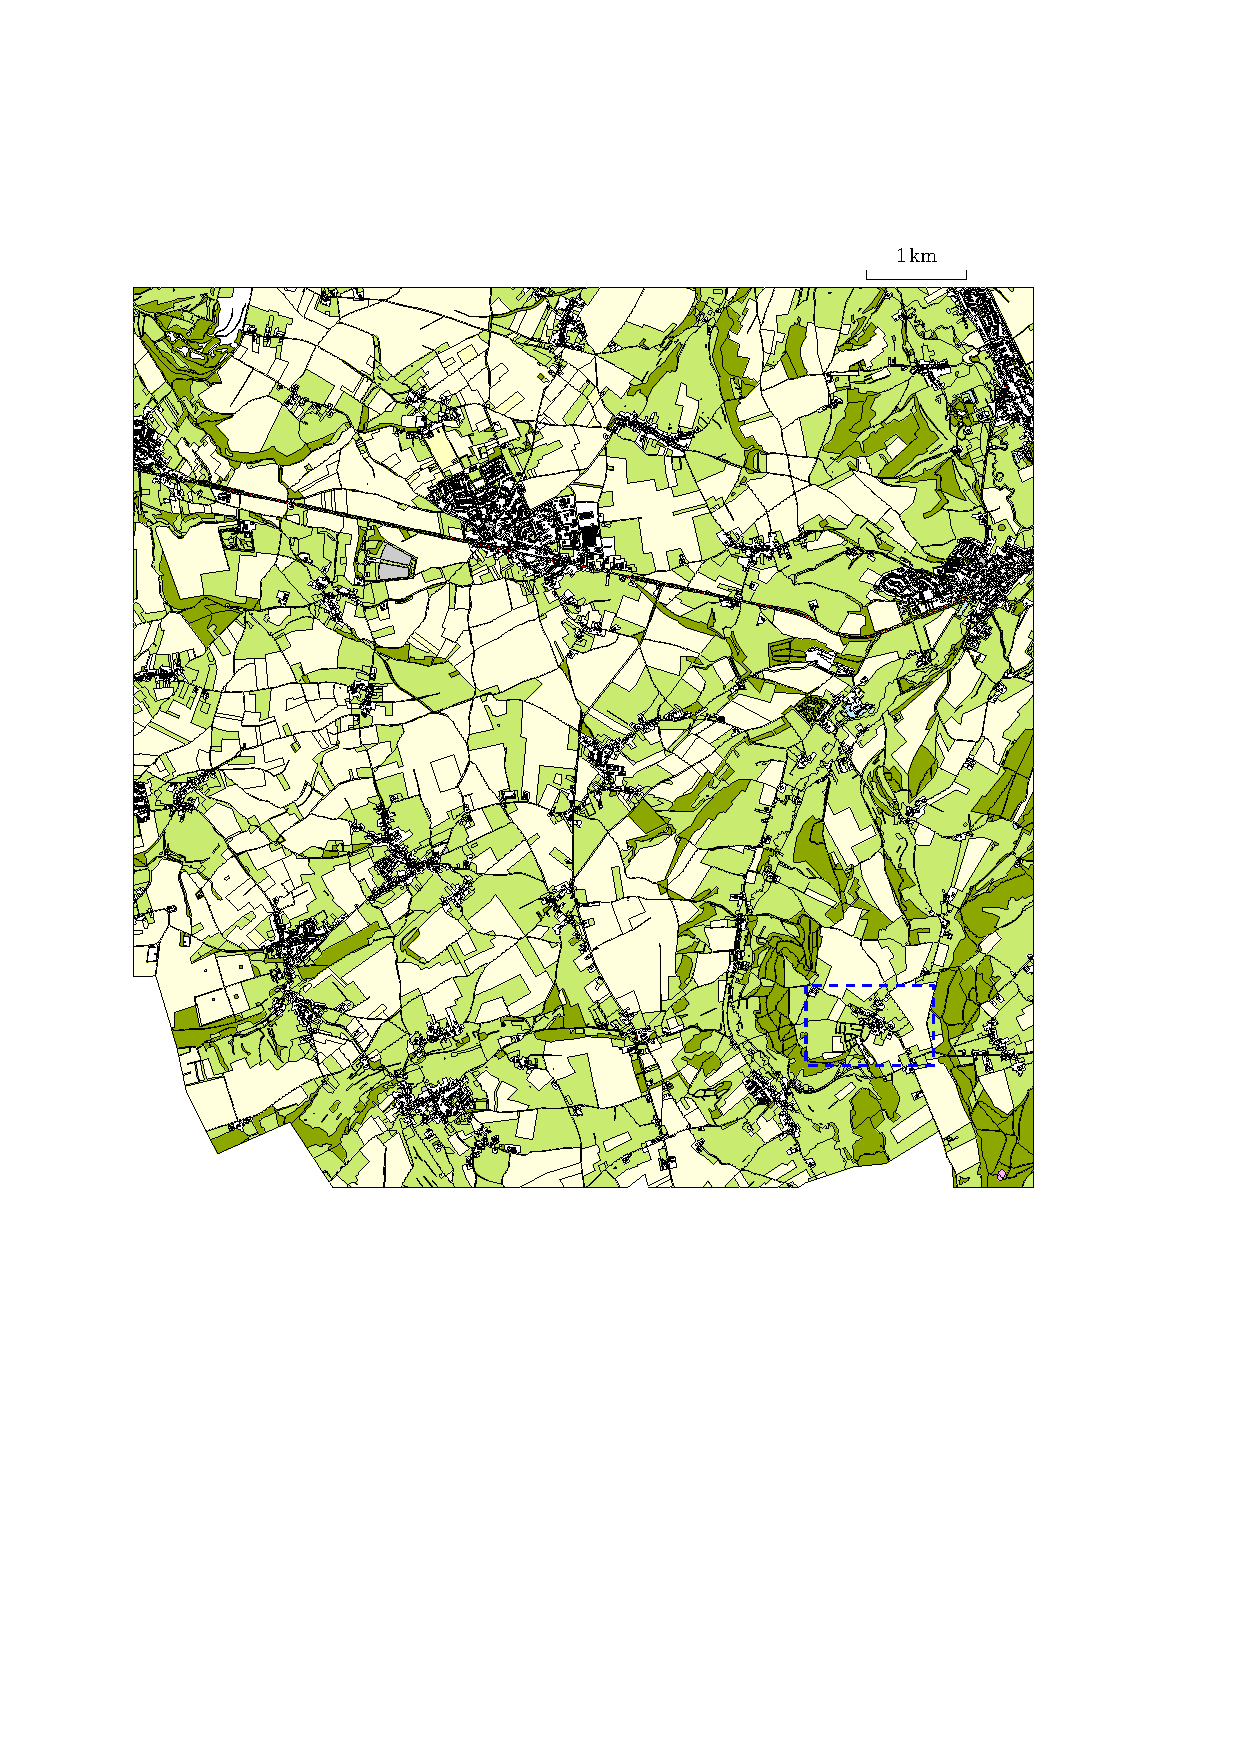
\includegraphics[page=1,draft=false,width=\linewidth,clip=true, trim = 12mm 14mm 2mm 0mm]{data}
\caption{
    The topographic map represents the place 
    in the south of Limburg, The Netherlands.
    There are $13{,}238$ parcels.
    The map is for scale $1:10{,}000$.}
\label{fig:data}
\end{figure}


\begin{figure}[tb]
\centering
\begin{subfigure}[t]{\textwidth}
\centering
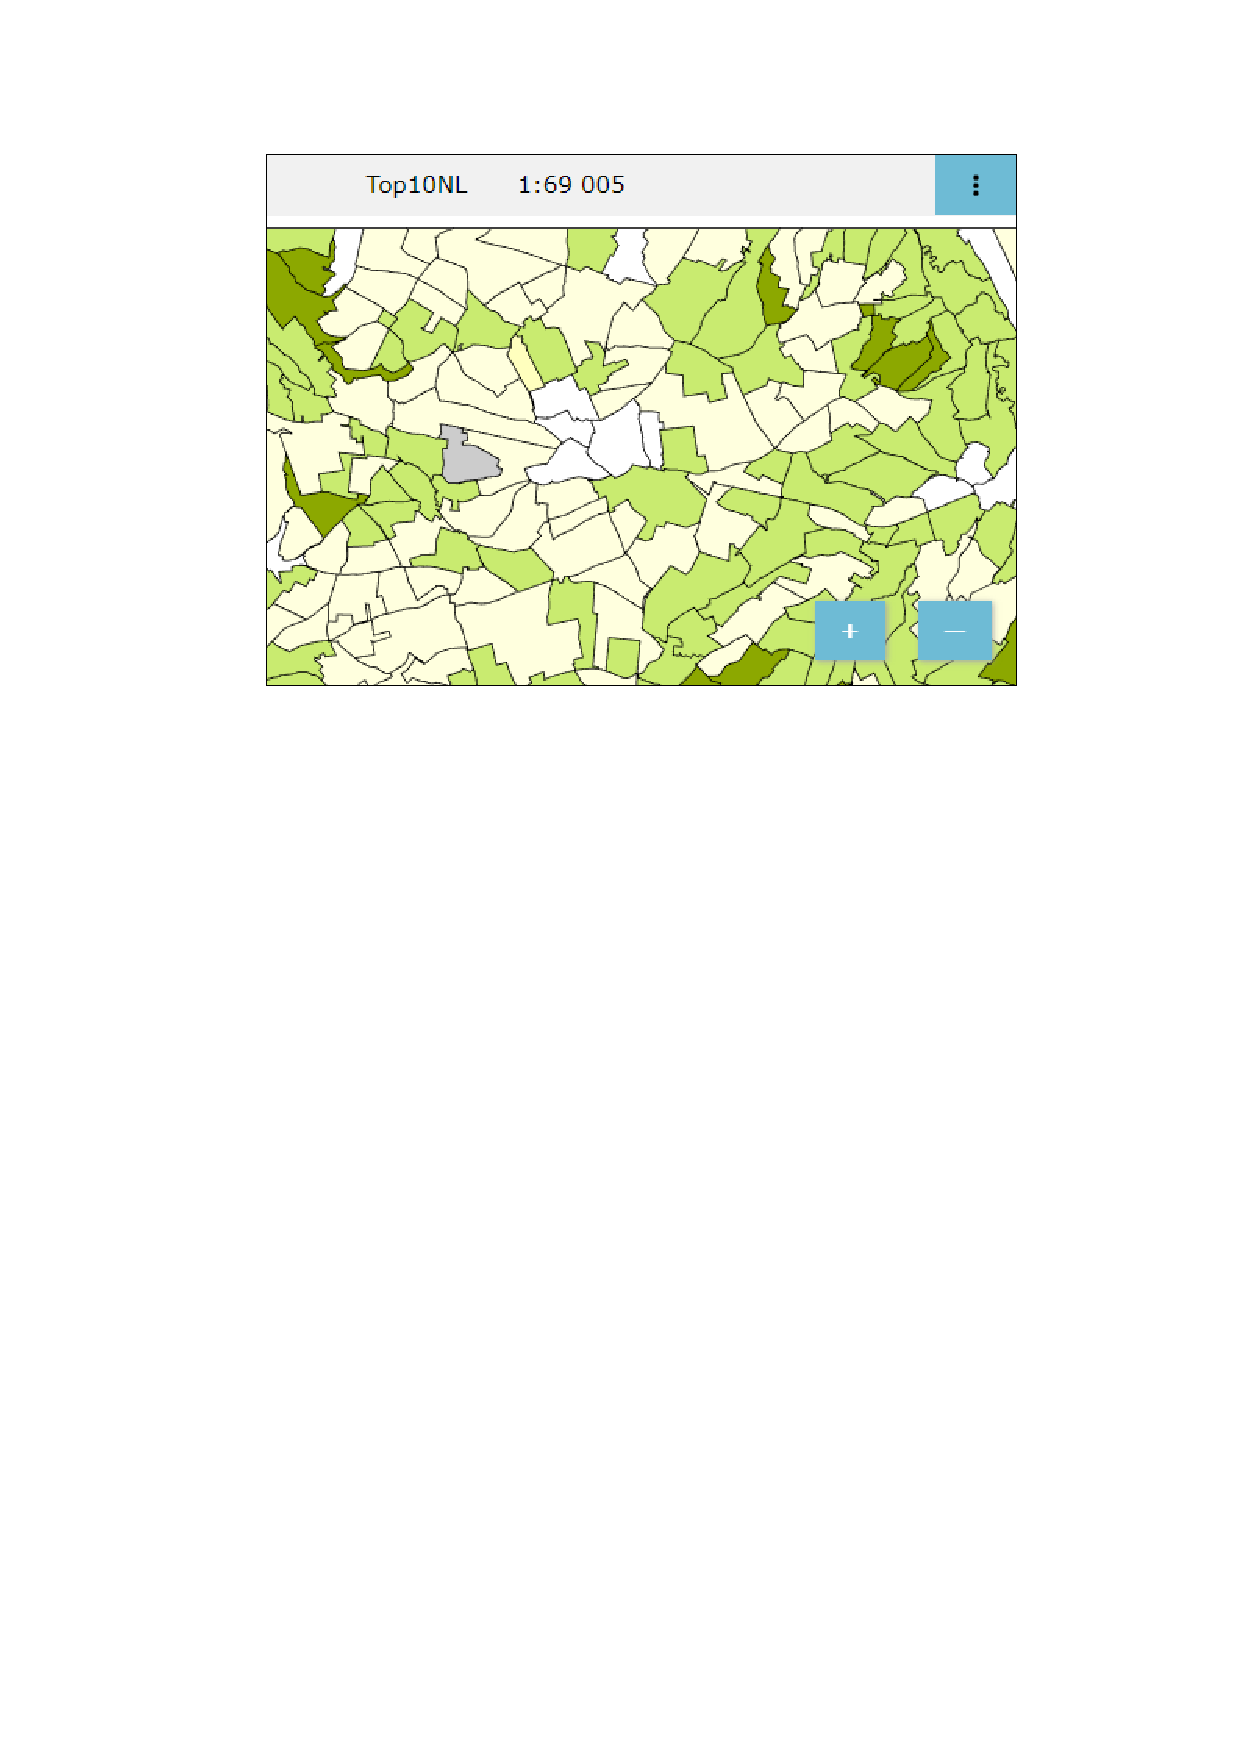
\includegraphics[page=1]{case_study}
\caption{An overview map. The map is generated from the base map 
    by parallel merging with parameter~$r_\mathrm{parallel}= 0.01$.}
\end{subfigure}
\newline
\vspace{0.5cm}
%
\begin{subfigure}[t]{\textwidth}
\centering
\includegraphics[page=2]{case_study}
\caption{A part of the base map. The displayed place is marked 
    by the dashed rectangle in \fig\ref{fig:data}.}
\end{subfigure}
\caption{Two examples of our web map with different scales.
    }
\label{fig:web_map}
\end{figure}

Some statistics of the results when 
parallel parameter~$r_\mathrm{parallel}=0.001$, $0.01$, or $0.1$ 
are shown in \tabl\ref{tbl:parallel_param_comparison}.
According to column~$N_\mathrm{step}$,
the number of steps decreases 
when the parallel parameter increases.
This is reasonable because more areas will be merged in each step.
As explained in \sect\ref{sec:greedy_algo}, 
for each merging step we iteratively select the least important area 
and its most compatible neighbor to define a merging event; 
then, we block the neighbors of the two areas.
Sometimes, a least important area is already blocked 
because of the previously found events.
This situation happens~$2{,}714$ times in total for all the steps
when parallel parameter~$r_\mathrm{parallel}=0.01$
(see column~$N_\mathrm{blocked}$ of \tabl\ref{tbl:parallel_param_comparison}).
%
Sometimes, although a least important area is free, 
its most compatible neighbor has been blocked 
because of the previously found events.
This case happens~$1{,}383$ times in total for all the steps
when parallel parameter~$r_\mathrm{parallel}=0.01$
(see column~$n_\mathrm{nbr\_blocked}$ of \tabl\ref{tbl:parallel_param_comparison}).
%
According to the statistics, we encounter more cases of the areas blocked
when merging a larger proportion of the area objects.
However, we can still reach our target number of events perfectly 
for settings of~$r_\mathrm{parallel}=0.01$ or~$r_\mathrm{parallel}=0.001$. 
Only when we push beyond the limit (\eg~$r_\mathrm{parallel}=0.1$), 
we can not reach the target number of events in a step 
(and we need correction information 
to compute the actual number of achieved events). 
When the target number of events cannot be met, 
one could also question the cartographic quality 
if there is hardly any free choice when generalizing.


\begin{table}[tb]
\centering
\caption{Some statistics when different parallel parameters area used 
    (\ie~$r_\mathrm{parallel}=0.001$, $0.01$, and $0.1$).
    Column~$N_\mathrm{step}$ records the number of steps to transit 
    from the base map to the map with a single area.    
    Column~$N_\mathrm{blocked}$ records the number of times
    when the least important area was blocked.
    Column~$N_\mathrm{nbr\_blocked}$ records the number of times 
    when the most compatible neighbor was blocked.
}
\begin{tabular}{rrrr}
\toprule
$r_\mathrm{parallel}$   & $N_\mathrm{step}$ & $N_\mathrm{blocked}$  & $N_\mathrm{nbr\_blocked}$ \\ \midrule
0.001                   &  3{,}195          &       211             &       72                  \\
0.01                    &  544              &   2{,}714             &  1{,}383                  \\
0.1                     &  91               & 100{,}617             & 34{,}268                  \\ 
\bottomrule 
\end{tabular}
%\begin{tabular}{cccc}
%\hline
%$r_\mathrm{parallel}$ & 0.001       & 0.01          & 0.1    \\ \hline
%eventdiff\_repetition & [[0, 3195]] & [[0, 544]]    & $L_{\mathrm{diff\_rep}, 0.1}$   \\
%least face blocked    & 228            & 3{,}216         & 105{,}980       \\
%best neighbor blocked & 72            & 1{,}841        & 38{,}232 \\ \hline 
%\end{tabular}
%\begin{Verbatim}[fontfamily=normal,commandchars=\\\{\},
%codes={\catcode`$=3\catcode`^=7\catcode`_=8}]
%\hspace{4cm}$L_{\mathrm{step\_eventdiff},0.1}$ = [[1, 53], [2, 138], $\dots$, [88, 1]]
%\end{Verbatim}
%\fvset{gobble=2}
%\begin{Verbatim}[fontfamily=normal,frame=single,
%label=$L_{\mathrm{diff\_rep}, 0.1}$]
%   [[51, 1], [138, 1], [152, 1], [200, 1], [205, 1], [181, 1], [198, 1], [167, 1], [173, 1], [165, 1], 
%    [153, 1], [143, 1], [140, 1], [127, 1], [125, 1], [108, 1], [103, 1], [92, 2], [84, 1], [79, 1], [74, 1], [68, 1], 
%    [60, 1], [54, 1], [46, 1], [50, 1], [48, 1], [45, 1], [39, 1], [44, 1], [37, 1], [36, 1], [32, 1], [30, 1], [26, 1], 
%    [28, 1], [21, 2], [18, 1], [20, 1], [16, 1], [12, 1], [13, 1], [8, 1], [12, 2], [6, 1], [12, 1], [11, 1], [8, 1], [7, 1], 
%    [6, 1], [7, 1], [4, 1], [5, 1], [4, 1], [5, 2], [7, 1], [5, 1], [4, 1], [5, 1], [3, 1], [4, 1], [3, 3], [2, 2], [1, 2], [2, 1], 
%    [1, 2], [2, 1], [1, 3], [0, 2], [1, 2], [0, 14]]
%\end{Verbatim}
\label{tbl:parallel_param_comparison}
\end{table}



As we can find the target numbers of merging events for all the steps
when parallel parameter~$r_\mathrm{parallel}= 0.001$ or~$0.01$, 
the corresponding exceptions lists are empty.
%For example, when~$r_\mathrm{parallel}= 0.01$,
%The content of the JSON file is as following.
%\begin{verbatim}
%                {
%                    "face_num": 13238,
%                    "parallel_param": 0.01,                    
%                    "step_eventdiff": []
%                }
%\end{verbatim}
When~$r_\mathrm{parallel}= 0.1$,
the exception list is~$[[1, 1304], [2, 1070], \dots, [77, 2]]$,
which has~$71$ pairs of values.
In reality, we would not use~$r_\mathrm{parallel}= 0.1$
(merging~$10\%$ of the current areas in every step)
because it is an unrealistic high value.
Using such a high value results in a multi-scale representation
(because we have a few valid states or scales),
whereas we would like to have representations at nearly
arbitrary scales.

%Important note: this is for a small subset 9x9 out of the 300x300 km^2 (whole country). To have same effect can we keep the r_parellel at same value, but we will have less situation where the target is not reached (more options)



We set zooming factor~$f_\mathrm{zoom}=1$ and 
zooming duration~$t_\mathrm{zoom}=1 s$ 
(see \sect\ref{sec:zooming_duration}).
When zooming on our web maps with different parallel parameters,
we observed that the impressions of the maps 
based on single merging\footnote{%
See the web map at
\url{https://congengis.github.io/webmaps/2020/05/merge/single-merging/}.} 
and based on parallel merging with parameter~$r_\mathrm{parallel}= 0.001$ 
are almost the same.
The reason is that the smooth merging happens too fast,
and we cannot really see the merging animation.
We get the feeling of smooth merging when~$r_\mathrm{parallel}= 0.01$.
When~$r_\mathrm{parallel}= 0.1$, the smooth merging is already obvious.
In order to show a better comparison of single merging 
and parallel merging,
we put two maps together (see \fig\ref{fig:comparison}),
where the parallel parameter is~$0.1$.\footnote{%
See the map of comparison at
\url{https://congengis.github.io/webmaps/2020/05/merge/0.1/comparer.html}.}  


\begin{figure}[tb]
\centering
\includegraphics[page=3]{case_study}
\caption{
    The map to the left of the slider is based on single merging,
    and the one to the right is based on parallel merging
    with~$r_\mathrm{parallel}= 0.1$.
    The slider can be moved to tune the widths of the two map canvases.
    The two maps are very different, and 
    we can observe some sudden changes across the slider.
}
\label{fig:comparison}
\end{figure}

When parallel parameter~$r_\mathrm{parallel}$ is set to~$0.1$,
we noticed a problem in the northeastern corner of the map.
That is, some tiny and relatively unimportant areas stay 
until the scale is very small,
while they should be merged much earlier.
This is due to the fact that 
there are many buildings in the northeastern corner of the map.
When the buildings share the same surrounding area,
they become holes of the polygon.
In each step, only one of the buildings will be merged into the surrounding area
because an area is allowed to merge with only one area in each step.
In the meantime, the areas at other places of the map merge relatively fast
because we allow $10\%$ of the areas to be merged in each step.
Fortunately, we would not need to use such a big parallel parameter in reality.


%To fix the problem, we should allow a surrounding area 
%to merge with many of its holes in a single step.


\section{Concluding remarks}
\label{sec:concluding_remarks}

\subsection{Conclusion}
%For the first time, 
This paper investigates on paralleling generalization operations,
using the merging operation as a case study. 
The purpose of having parallel generalization operations 
is to have smoother zooming experience later on 
(compared to the pure sequenced individual generalization events)
so that users can better keep their context during zooming.
This paper develops a greedy algorithm to find parallel events of 
merging area objects.
Then, the parallel events are integrated into 
the tGAP and the SSC to nicely visualize the merging animations.
%This paper also proposed a strategy 
%to concisely store the number of merging events for all the steps.
To guarantee that the merging animations always complete for zooming, 
we managed to snap zooming operations to valid states.
This paper also presents a recipe 
to define the animation duration of an event.
According to our case study,
the events of parallel merging 
can be better observed than the events of single merging.
This result shows the potential that
users can keep their context better 
and can have smoother map interaction experience
when zooming on a map based on parallel-event operations.



\subsection{Future work}

Many topics related to this research need to be investigated further.
\fig\ref{fig:smooth_merging}a--e shows our solution of
gradually expanding an area over the other area.
It may be even better if the color of the smaller area (pink)
adapts to the color of the larger one (light yellow) smoothly
(see \fig\ref{fig:smooth_merging}f--j).


\begin{figure}[tb]
\centering
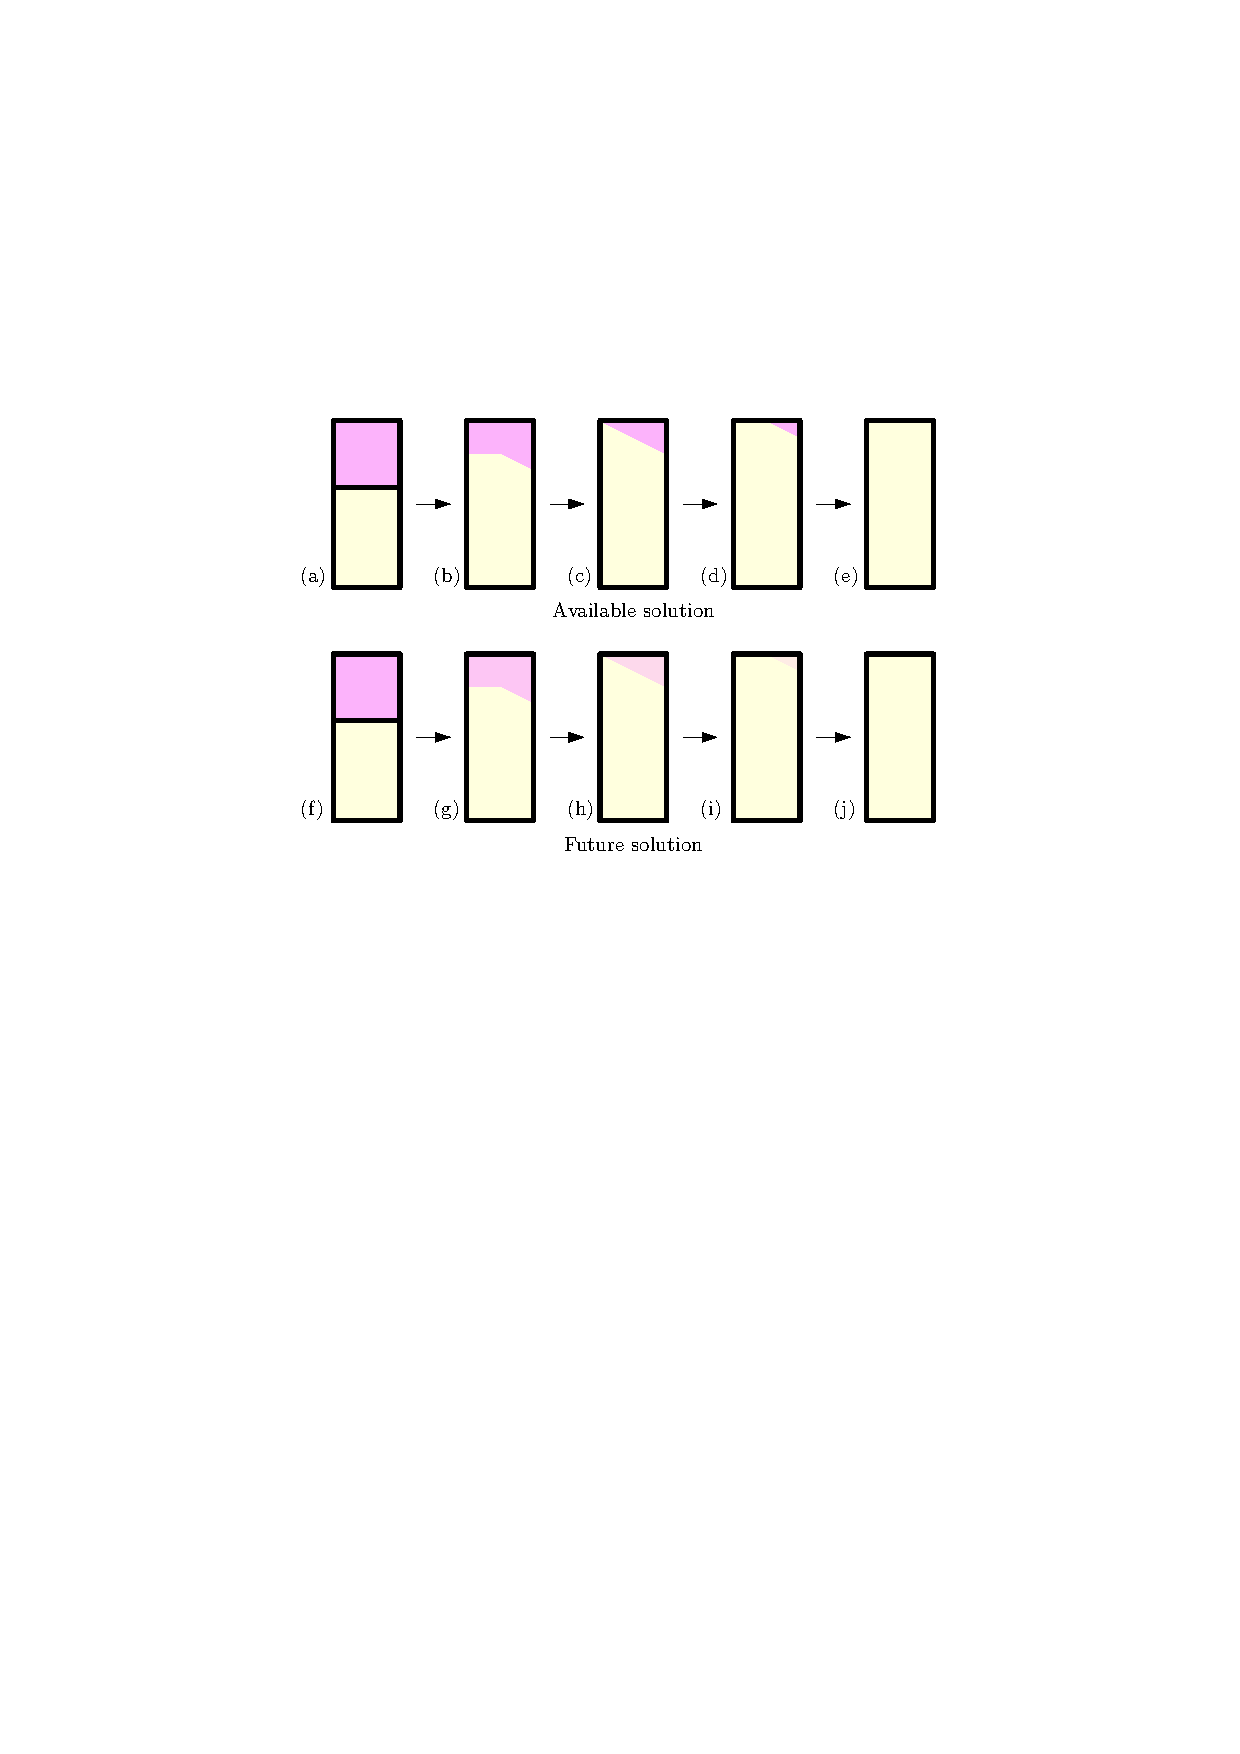
\includegraphics[page=1]{concluding_remarks}
\caption{
    Our available solution of merging animation 
    and a possible future solution.}
\label{fig:smooth_merging}
\end{figure}



%\begin{figure}[tb]
%\centering
%\includegraphics[page=1]{smooth_merging}
%\caption{A smooth way of merging two areas,
%    where the larger area gradually expands over the smaller one.}
%\label{fig:smooth_merging}
%%
%\vspace{6mm}
%%
%\centering
%\includegraphics[page=2, scale=0.3]{smooth_merging}
%\caption{The space-scale cube for the merging 
%    of \fig\ref{fig:smooth_merging}.
%    This figure is made by visualizing the content of an obj file in 
%    ParaView 5.6.0.}
%\label{fig:smooth_merging_ssc}
%\end{figure}




This paper used a greedy algorithm 
to find parallel merging events for each step.
Alternatively, it is possible to define merging steps 
by selecting and combining some single-event steps of a sequence found 
by some existing methods
(\eg~the greedy algorithm of \citet{vanOosterom2005}
or the \Astar algorithm of \citet[\chap2]{Peng2019Thesis}).

Currently, the merging events distribute randomly on a map.
If we are unlucky, there may be a lot of events 
happening in users' focused region for a zooming duration,
which may cause the users to lose track of their interested objects;
for another zooming duration, 
there may be no event happening in the focused region at all.
The strategy of blocking neighbor areas in our greedy algorithm 
already mitigates the problem.
However, it may be even better if 
we explicitly distribute the merging events evenly, 
then the workload for a user to follow the events is stable during the zooming.
To this end, we could divide a map into many regions 
using a field-tree-like, multiple-level grid \citep{vanPutten1998NewGAP}
or using the road network.
Then, we could find a certain number of events in each of the regions 
according to the regions' sizes,
which should result in an even distribution of events.
Finally, we could compare our current greedy algorithm and 
the algorithm considering even distribution.


Our current event consists of only the merging operation,
it is also necessary to involve split operation
because sometimes a merging operation results in an unnatural area.
For example, it is weird to merge a long and thin area 
with one of the areas that are along it
\citep[see][]{Haunert2008Skeleton}.
Therefore, such kind of long and thin areas should be
split into several parts first.
We may integrate a split method based on the straight skeleton
\citep{Haunert2008Skeleton}
or the skeleton obtained from a constrained Delaunay triangulation
\citep{Meijers2016Split}.
In addition to area features, we also need to support line features 
for these long objects (\eg~roads, river, rail) for the smaller scales.
In order to apply appropriate generalization operators
for a certain scale,
we need to extend and implement the framework 
to guide our generalization choices
\citep{Meijers2018Framework}.


To avoid clutter of vertices for zooming out, 
it is necessary to simplify the boundaries of the areas.
Many existing methods could be integrated into our parallel paradigm.
\citet{Meijers2011LineSimp} proposed a method 
to simplify the boundaries parallelly. 
Their results are topologically safe. 
Another choice would be the method of \citet{ImaiIri1988},
which is able to minimize the number of vertices 
for a given error threshold.
One more choice would be to construct compatible triangulations 
\citep[see][\chap3]{Peng2019Thesis}
for the two levels of topographic maps.
In the SSC, we could build some tilted walls 
to connect the two levels of compatible triangulations.
When we slice this SSC to animate a zooming action,
the boundaries of the areas are morphed 
(moved smoothly and parallelly)
between a detailed representation and a coarse representation.
We can imagine that it is challenging to build the tilted walls.
Furthermore, we would like to 
simplify point symbols and text labels in a smooth way.
For this purpose, we may need to integrate the ideas of
\citet{Haunert2017Label} and \citet{sahw-oarps-ICAGW13}.

We would also like to realize smooth zooming
between a foreground map and a background map,
which respectively present a thematic data and a topographical data.
When a user zooms in, the foreground map should be displayed,
and when the user zooms out,
the background map should be displayed.
Furthermore, we would like to 
integrate time dimension into our 3-dimensional SSC
to form a 4-dimensional space-scale-time structure (a tesseract).
Then, we have the opportunity to store all the updates along time in the tesseract.
By ``slicing'' it, we will be able to output a map at any scale and any time point.


This paper develops technique for smooth zooming based on parallel merging,
and we hope that it allows map users to follow the zooming more easily.
A future work is to investigate 
how much map users benefit from our technique.
We will conduct some usability tests based on the experience of
\citet[\sect6.7]{Suba2017Thesis} and \citet{Midtbo2007}.




%When we remove a triangle by slicing the SSC, 
%we may want to keep three vertices of the triangle 
%instead of making four vertices.
%In this case, the polyhedron (with five faces) should have curly edges,
%which is also known as a \emph{curved polyhedron}.
%The slopes of curly edges need to be studied.








%Some research questions are as follows.
%What aspects should we optimize 
%(\eg~minimizing the number of merging events or 
%assigning similar numbers of merging steps to each event)?
%What algorithm should we use 
%(\eg~dynamic programming, \Astar, or integer linear programming)?
%How much time is gained for users to observe the merging steps on the screen?
%How to store the parallel merging steps?




\section*{Data and codes availability statement}

The data and codes used in this case study 
can be found at \emph{figshare} 
(see \url{https://figshare.com/s/199e049e2a0f9c18d19a}).
The data was derived from open-access dataset TOP10NL,
which is a topographic map produced by Kadaster
(see \url{https://www.pdok.nl/downloads/-/article/basisregistratie-topografie-brt-topnl}).
%\footnote{%
%Dataset TOP10NL can be downloaded at
%\url{https://www.pdok.nl/downloads/-/article/basisregistratie-topografie-brt-topnl},
%accessed: May 17, 2020.}



%\section*{Acknowledgement(s)}
%We thank Radan Šuba for partly creating the data used in our case study.
%An unnumbered section, e.g.\ \verb"\section*{Acknowledgements}", may be used for thanks, etc.\ if required and included \emph{in the non-anonymous version} before any Notes or References.
%
%
%\section*{Disclosure statement}
%
%An unnumbered section, e.g.\ \verb"\section*{Disclosure statement}", may be used to declare any potential conflict of interest and included \emph{in the non-anonymous version} before any Notes or References, after any Acknowledgements and before any Funding information.
%
%
%\section*{Funding}
%
%This research is supported by the Netherlands Organisation for 
%Scientific Research (NWO, project number 17644), 
%which is partly funded by the Ministry of Economic Affairs.


%
%\section*{Notes on contributor(s)}
%
%An unnumbered section, e.g.\ \verb"\section*{Notes on contributors}", may be included \emph{in the non-anonymous version} if required. A photograph may be added if requested.
%
%
%\section*{Notes}
%
%An unnumbered `Notes' section may be included before the References (if using the \verb"endnotes" package, use the command \verb"\theendnotes" where the notes are to appear, instead of creating a \verb"\section").

\bibliographystyle{tfv}
\bibliography{Reference/BibReference}




\appendix

\section{Create the table of weights and the table of compatibility values}
\label{appx:create_tables}
This appendix shows how to create the table of weights and 
the table of compatibility values in PostgreSQL.
The values of the two tables are used in our greedy algorithm
(see \sect\ref{sec:greedy_algo}).
Currently, we have not investigated on 
how to define the weight for a class,
so we assign value~$1$ to the weights of all the classes.
That is to say, the least important area is the one with the smallest size.
The class similarity is defined based on the class codes 
as the codes indeed imply a hierarchy.

\bigskip

\lstinputlisting[
           language=SQL,
           showspaces=false,
           showstringspaces=false,
%           basicstyle=\ttfamily,
%           basicstyle=\small,
           basicstyle=\footnotesize,
%           numbers=left,
%           numberstyle=\tiny,
           commentstyle=\color{gray},
           linewidth=\textwidth,
           gobble=2,
           tabsize=2,
        ]{images/top10nl_9x9_class_comp_weight_tabes.sql}

\bigskip

\section{Communicate valid states}
\label{appx:communicate_valid_states}

\sect\ref{sec:snap} shows how to snap to only valid states 
to avoid half-way merging.
This appendix illustrates how to communicate valid states 
from the server side to the client side.
By sending only the exceptions of the event number, 
we try to decrease the size of the sent data.



\subsection{On the server side}
\label{sec:communicate_server}

On the server side, 
we compute the values shown in \tabl\ref{tbl:sequence_greedy}.
These values are for merging sequence of \fig\ref{fig:intro}k--o 
(also see \tabl\ref{tbl:face_tgap}b),
where parallel parameter~$r_\mathrm{parallel}$ was set to~$0.3$.
Note that this parameter value is extremely high, 
just used to explain the principle in an artificial simple example.
The computation starts from step~$1$.
At the beginning, there are $7$ areas on the map, \ie~$|M_0| = 7$.
According to \eq\ref{eq:n_target},
our target is to parallel three events ($n_{\mathrm{target},1} = 3$).
However, only two event can be paralleled in step~$1$ 
because some areas are blocked
(see \fig\ref{fig:blocked_polygons}b).
Therefore, we have~$n_{\mathrm{event},1} = 2$.
%The difference of the target value and the real value
%can be computed by
%\begin{equation}
%\label{eq:n_diff}
%n_{\mathrm{diff},i} = n_{\mathrm{target},i} - n_{\mathrm{event},i},
%\end{equation}
%where variable~$i$ indicates the $i$-th step.
%That is, we have~$n_{\mathrm{diff},1}=1$, for step~$1$
%(also see the $n_\mathrm{diff}$ value in the first row of \tabl\ref{tbl:sequence_greedy}).
We require that the low state is~$s_{\mathrm{low},1} = 0$ for the first step.
Then, the $s_\mathrm{high}$ value can be computed by
\begin{equation}
\label{eq:state_high}
s_{\mathrm{high},i} = s_{\mathrm{low},i} + n_{\mathrm{event},i}.
\end{equation}
That is, we have~$s_{\mathrm{high},1}=2$
(also see the~$s_\mathrm{high}$ value in the first row of \tabl\ref{tbl:sequence_greedy}).
At this point, the computation for step~$1$ completes.


\begin{figure}[h]
%\centering
%\includegraphics[page=2]{blocked_polygons}
%\caption{.
%}
%\label{fig:sequence_greedy}
%\vspace{6mm} %for some reason, the space below the caption is not enough
%
%
%
\captionsetup*{type=table} %*: suppress warning "The caption type was already set to figure"
\caption{Some information of the merging sequence shown in \tabl\ref{tbl:sequence_greedy}.
Column~$n_\mathrm{area}$ shows the area number of the map at starting state~$s$,
that is, $|M_s|$ of \eq\ref{eq:n_target}.
}
\label{tbl:sequence_greedy}
\centering
\begin{tabular}{cccccc}
\toprule
step & $n_\mathrm{area}$ & $n_\mathrm{target}$ 
& $n_\mathrm{event}$ & $s_\mathrm{low}$ & $s_\mathrm{high}$ \\ \midrule
1        & 7      & 3        & 2        & 0      & 2      \\
2        & 5      & 2        & 2        & 2      & 4      \\
3        & 3      & 1        & 1        & 4      & 5      \\
4        & 2      & 1        & 1        & 5      & 6      \\
%5        & 2      & 1        & 1        & 0     & 5      & 6      \\
%6     & 1      & ---      & ---      & ---    \\ 
\bottomrule
\end{tabular}
\end{figure}

For the next step, the number of areas can be computed by
$$
n_{\mathrm{area},i+1} = n_{\mathrm{area},i} - n_{\mathrm{event},i},
$$
where variable~$n_{\mathrm{area},i}$ denotes the area number 
at the low state of step~$i$.
Furthermore, the state-low value of step~$i+1$ (\ie~$s_{\mathrm{low},i+1}$) 
is the same as the state-high value of step~$i$ (\ie~$s_{\mathrm{high},i}$).
Again, the target number of parallel events (\ie~$n_{\mathrm{target},i+1}$)
is computed by \eq\ref{eq:n_target},
the number of actual parallel events is obtained from the greedy algorithm,
%the value of difference (\ie~$n_{\mathrm{diff},i+1}$) 
%is computed by \eq\ref{eq:n_diff}, 
and the state-high value (\ie~$s_{\mathrm{high},i+1}$) 
is computed by \eq\ref{eq:state_high}.
The computation of all the steps starts from step~$i=1$ and 
finishes until only one area left on the map.
As a result, we have all the values of \tabl\ref{tbl:sequence_greedy}.


%Then the difference in step~$i$ is
%\begin{equation}
%\label{eq:n_diff}
%n_{\mathrm{diff},i} = n_{\mathrm{target},i} - n_{\mathrm{event},i},
%\end{equation}
%where variables~$n_{\mathrm{target},i}$ and~$n_{\mathrm{event},i}$
%are respectively the expected and the real numbers of events in step~$i$,
%which are consistent with the definitions of 
%\eqs\ref{eq:n_target} and~\ref{eq:n_event_state}.
%For the next step, we compute
%$$
%n_{\mathrm{area},i+1} = n_{\mathrm{area},i} - n_{\mathrm{event},i},
%$$
%where variable~$n_{\mathrm{area},i}$
%represents the area number at the starting state of step~$i$.
%Based on number~$n_{\mathrm{area},i+1}$,
%we can further compute $n_{\mathrm{target},i+1}$ and obtain $n_{\mathrm{event},i+1}$.
%This process starts from step~$i=1$ and ends until only one area left.

Now, we have a column of~$n_\mathrm{event}$ values.
Among them, we record the exceptions 
(\ie~when value~$n_\mathrm{event}$ is different from value~$n_\mathrm{target}$) 
with the corresponding steps in a list.
The \emph{exception list} is~$[[1, 2]]$ for the example of \tabl\ref{tbl:sequence_greedy}.
For the pair of values in the inner square brackets,
the first one represents the step,
and the second value represents the actual number of events~$n_\mathrm{event}$.
The exception list, the number of faces, and the parallel parameter 
will be sent to the client side.
 
%Take \tabl\ref{tbl:sequence_greedy} for example,
%the list is $[[1, 1]]$.
%The content of the JSON file is as following.
%\begin{verbatim}
%                {
%                    "face_num": 7,
%                    "parallel_param": 0.3,                    
%                    "step_eventdiff": [[1, 1]]
%                }
%\end{verbatim}


%We compress those values as the form of 
%$$
%[[n_{\mathrm{diff},1},j_1], [n_{\mathrm{diff},1+j_1},j_2], \ldots, 
%[n_{\mathrm{diff},i},j_k], [n_{\mathrm{diff},i+j_k},j_{k+1}], \ldots],
%$$
%where variable~$j_k$ is the number of the same $n_\mathrm{diff}$ values in a row 
%starting at step~$i$.
%Take \tabl\ref{tbl:sequence_greedy} for example, 
%the value of~$j_1$ is~$1$
%because the following value (\ie~0) is already different 
%from the first value (\ie~1) of~$n_\mathrm{diff}$.
%The value of~$j_2$ is~$3$ 
%because there are three same values in a row (\ie~0). 
%According to our strategy, 
%the~$n_\mathrm{diff}$ values of \tabl\ref{tbl:sequence_greedy}
%will be compressed to~$[[1,1], [0,3]]$,
%where each pair of values in the inner square brackets 
%record an~$n_\mathrm{diff}$ value and the number of repeat times.
%The content of the JSON file is as following.
%\begin{verbatim}
%                {
%                    "face_num": 7,
%                    "parallel_param": 0.3,                    
%                    "step_eventdiff": [[1, 1]]
%                }
%\end{verbatim}
%If we would have a list of $n_\mathrm{diff}$ values~$[0, 0, 0, 0, 0, 0, 5, 0, 0]$,
%then the compressed content would be~$[[0,6], [5,1], [0,2]]$.
%Our case study will show that this way of compressing is efficient
%(see \sect\ref{sec:case_study}).



\subsection{On the client side}
\label{sec:communicate_client}


When a user opens our web map,
the client side receives the exception list, the number of faces, 
and the parallel parameter from the server side.
%the JSON file will be sent to the client side.
%We can unpack the content of entry ``step\_eventdiff'' and 
%get the list of $n_\mathrm{diff}$ values~$[1, 0, 0, 0]$.
Starting from step~$i=1$,
we see if the step is in the exception list.
If so, the event value of step~$i$ from the list 
is assigned to~$n_{\mathrm{event},i}$.
If not, value~$n_{\mathrm{target},i}$ (see \eq\ref{eq:n_target})
is computed and assigned to~$n_{\mathrm{event},i}$.
%where parallel parameter~$r_\mathrm{parallel}=0.3$ 
%and face number~$n_{\mathrm{area},1} = 7$
%can be obtained also from the JSON file.
%Then, we can compute the actual number of parallel events by
%\begin{equation*}
%\label{eq:n_event_step}
%n_{\mathrm{event},i} = n_{\mathrm{target},i} - n_{\mathrm{diff},i},
%\end{equation*}
%where value~$n_{\mathrm{diff},i}$ is~$0$ if no value of step~$i$
%exists in the exception list.
%Note that \eq\ref{eq:n_event_step} 
%is an inverse function of \eq\ref{eq:n_diff}.
As a result, we have the~$n_\mathrm{event}$ values on the client side
(see column~$n_\mathrm{event}$ in \tabl\ref{tbl:sequence_greedy}).
By accumulating the~$n_\mathrm{event}$ values,
we obtain the list of valid states~$S_\mathrm{valid} = [0, 2, 4, 5, 6]$.



\end{document}
